\documentclass[5p,twocolumn,authoryear]{elsarticle}
\usepackage[T1]{fontenc}
\usepackage{lmodern}
\setlength{\emergencystretch}{1em}
\usepackage{amsmath,amssymb,booktabs,graphicx,array,microtype}
\usepackage{xcolor,hyperref}
\usepackage{dblfloatfix}
\renewcommand{\topfraction}{0.95}
\renewcommand{\dbltopfraction}{0.95}
\renewcommand{\textfraction}{0.05}
\renewcommand{\floatpagefraction}{0.75}
\renewcommand{\dblfloatpagefraction}{0.75}
\setcounter{dbltopnumber}{2}
\usepackage{tikz}
\usetikzlibrary{arrows.meta,positioning,fit,backgrounds}
\hypersetup{colorlinks=true,linkcolor=blue!50!black,citecolor=blue!50!black,urlcolor=blue!50!black}
\newcommand{\todo}[1]{\textcolor{red!70!black}{[TO COMPLETE: #1]}}
\newcommand{\nojepa}{\textsc{NoJEPA}}
\newcommand{\direct}{\textsc{DirectReadout}}
\newcommand{\fullmodel}{\textsc{ForecastMean}}
\journal{Medical Image Analysis}
\begin{document}
\begin{frontmatter}
\title{Forecast-aware latent modeling for longitudinal prediction of pathological complete response from breast MRI}
\author{Author information to be completed}
\address{Affiliations and corresponding author to be completed}
\begin{abstract}
Longitudinal breast MRI can reveal treatment response, but endpoint classifiers do not explicitly model the future trajectory implied by an observed history. We investigate forecast-aware latent modeling for pathological complete response (pCR) prediction using three-phase dynamic contrast-enhanced MRI, baseline clinical variables, and assigned-arm scenarios. An autonomous predictor estimates future latent states. A mean readout combines spatial arithmetic means of the predicted terminal state and its change with direct history features. The cohort comprises 976 patients and 3,641 examinations, with 801 development patients and a fixed internal holdout of 175 patients, including 56 positive outcomes. Three principal models distinguish prediction without future-state supervision, auxiliary-supervised direct prediction, and explicit forecast-mean readout. We evaluate training seeds 42, 44, 71, and 2026, averaging five fold probabilities within each seed before computing metrics and then equally averaging seed-specific metrics. Forecast mean achieved T0/T1/T2 AUROCs of 0.7476/0.7494/0.7478 and Macro AUROC/AP/F1 of 0.7483/0.6197/0.5760, compared with 0.7258/0.5905/0.5382 for the control without future-state supervision. Its Macro AUROC sample seed standard deviation was 0.0067. The full-versus-control AUROC difference was +0.0225, with approximate paired-bootstrap $p=0.00050$, nine-test Holm $p=0.00450$, and all-78 Holm $p=0.03850$. Macro AP and F1 differences did not pass principal-family adjustment. The T2 AUROC all-test conclusion crossed the 0.05 threshold in a larger independent Monte Carlo sensitivity check. Forecast mean had higher sensitivity but lower specificity and worse probability-quality point estimates than auxiliary-supervised direct readout. The overall-model and seed choices were retrospective; these conditional internal findings require independent validation and prospectively fixed evaluation policies.
\end{abstract}
\begin{keyword}
Breast MRI \sep Pathological complete response \sep Longitudinal imaging \sep Latent dynamics \sep Treatment response prediction
\end{keyword}
\end{frontmatter}
\section{Introduction}
\label{sec:intro}
Neoadjuvant systemic therapy provides an opportunity to monitor breast cancer before surgery and to study how an individual tumor responds over time. Pathological complete response (pCR) is a clinically meaningful endpoint associated with long-term outcomes, although its relationship to prognosis varies across biological subtypes and it should not be equated with a universally valid trial-level surrogate \citep{ctneobc2014}. Predicting pCR from imaging could support response assessment and the design of future adaptive studies. Such a prediction remains a prognostic estimate under an observed treatment context; it does not establish that changing treatment would improve an individual patient's outcome.

Dynamic contrast-enhanced MRI captures three-dimensional anatomy and contrast uptake patterns that evolve during therapy. Prior work in the I-SPY setting has demonstrated associations between MRI-derived tumor measurements and pathological response or subsequent outcomes \citep{hylton2012mri,hylton2016ftv}. Public multicenter imaging resources also make it possible to examine learned representations across repeated visits \citep{tciaispy2_2022,tciaacrin6698_2021}. However, a longitudinal prediction system must operate at the time a decision is considered: a baseline prediction can use baseline information, whereas an interim prediction can use the examination history accumulated by that interim visit. Future scans may inform representation learning on development patients but cannot become inputs to predictions for holdout patients at an earlier landmark.

Most direct classifiers optimize the endpoint of interest from observed images and clinical variables. This is a reasonable objective, but it does not explicitly require the representation to capture how the tumor state may evolve. A different strategy is to predict future imaging information and use the prediction to inform the endpoint readout. Image synthesis provides one route to such a representation, but prediction in a compact latent space can focus the training signal on state evolution without requiring a pixel-space image generator at inference. This distinction is useful for response prediction: the relevant question is whether the learned forecast contributes information to classification, rather than whether a generated image is visually convincing.

Joint-embedding predictive learning offers a general mechanism for predicting target representations computed by a slowly updated encoder \citep{jepa2023}. In a longitudinal medical setting, adapting that principle requires explicit handling of partial histories, missing future observations, treatment context, and the distinction between an auxiliary training target and a classifier input. A model may benefit from a future-state loss while still making a direct prediction from the observed history. Conversely, directly including forecast features in the classifier changes both its information pathway and its parameterization. These effects should be examined through matched controls rather than attributed to a single generic ``world model'' component.

We investigate forecast-aware latent modeling for longitudinal pCR prediction from breast MRI. The model encodes three selected DCE phases at each available visit, fuses observed MRI with baseline clinical information and an assigned treatment-arm scenario, and autonomously rolls the current latent state forward to a terminal stage. Spatial arithmetic means summarize the predicted terminal state and its change from the current state for pCR classification. We compare the complete model with two direct-readout controls: one without future-state supervision and one with the same auxiliary supervision as the complete model.

The study makes three concrete contributions. First, it formulates a common representation and masked future-state objective that can be applied to available T0--T2 histories while using observed later scans only as development-time targets. Second, it provides a staged comparison that distinguishes the effect of auxiliary prediction from the joint effect of forecast-feature readout and classifier parameterization. Third, it reports landmark-specific discrimination, class-specific errors, calibration, hypothetical decision curves, subgroup heterogeneity, archived forecasting diagnostics, and paired patient-level uncertainty on a fixed internal holdout. The manuscript evaluates each variant with training seeds 42, 44, 71, and 2026. Five fold probabilities are averaged within each seed before computing metrics; the metric values are then equally averaged across seeds and accompanied by descriptive seed standard deviations. The choice of mean forecast readout as the overall model, this seed set, and the aggregation policy were selected retrospectively, and patient-level inference conditions on the selected fitted predictors. Seed-selection and upstream-independence limits remain explicit.

\section{Related work}
\label{sec:related}
\paragraph{MRI biomarkers and learned pCR prediction.}
MRI-based response assessment has a substantial clinical and quantitative foundation. Functional tumor volume and related measurements have been studied in longitudinal breast MRI cohorts, including I-SPY \citep{hylton2012mri,hylton2016ftv}. The ACRIN 6698 study additionally examined diffusion-derived measurements in relation to response \citep{ACRIN6698diffusion2018}. These studies motivate imaging-based monitoring but do not establish that a learned model using different inputs or a different evaluation split has equivalent clinical validity. Our experiments use selected DCE phases and baseline clinical variables; diffusion imaging is not an input to the present model.

Learning-based approaches can combine complementary image sequences or repeated examinations. Synthesis-based representation learning has been explored for multi-sequence 3D/4D MRI \citep{han2024synthesis}, and recent studies have examined spatiotemporal or early-treatment information for pCR prediction \citep{tang2025spatiotemporal,du2025early}. Such studies provide relevant methodological context, but differences in patient selection, imaging availability, endpoints, and holdout construction prevent direct numerical comparisons with our results. We therefore do not claim superiority to published systems from cross-paper metric comparisons. Reimplementation of suitable external baselines under the same patient split remains necessary.

\paragraph{Predictive latent representations.}
Predicting a target embedding rather than reconstructing the input image is a central idea in joint-embedding predictive learning \citep{jepa2023}. We use an exponential-moving-average target encoder to define latent states and supervise autonomous future predictions. The present objective is a supervised pCR loss combined with a masked multi-step latent-state loss. It does not activate a separate single-step teacher-forcing JEPA loss, image reconstruction loss, or latent-variance regularizer. This objective-level distinction matters when interpreting the internal experiment name \nojepa{}: that control removes future-state supervision, while retaining the common fusion architecture.

\paragraph{Attention and volumetric image representation.}
Transformer attention provides a flexible way to combine image tokens and contextual information \citep{vaswani2017}. Compact convolutional representations can reduce the cost of processing volumetric MRI, and vector-quantized generative models provide one source of pretrained convolutional encoders \citep{vqgan2021}. Here the pretrained codec contributes a continuous convolutional encoder. The quantizer and image decoder are bypassed, and the main experiments do not synthesize MRI volumes. The final attention weights summarize latent tokens that have already undergone spatial mixing; they are therefore not validated lesion segmentations or anatomical explanations.

\section{Method}
\label{sec:method}
\begin{figure*}[t]
\centering
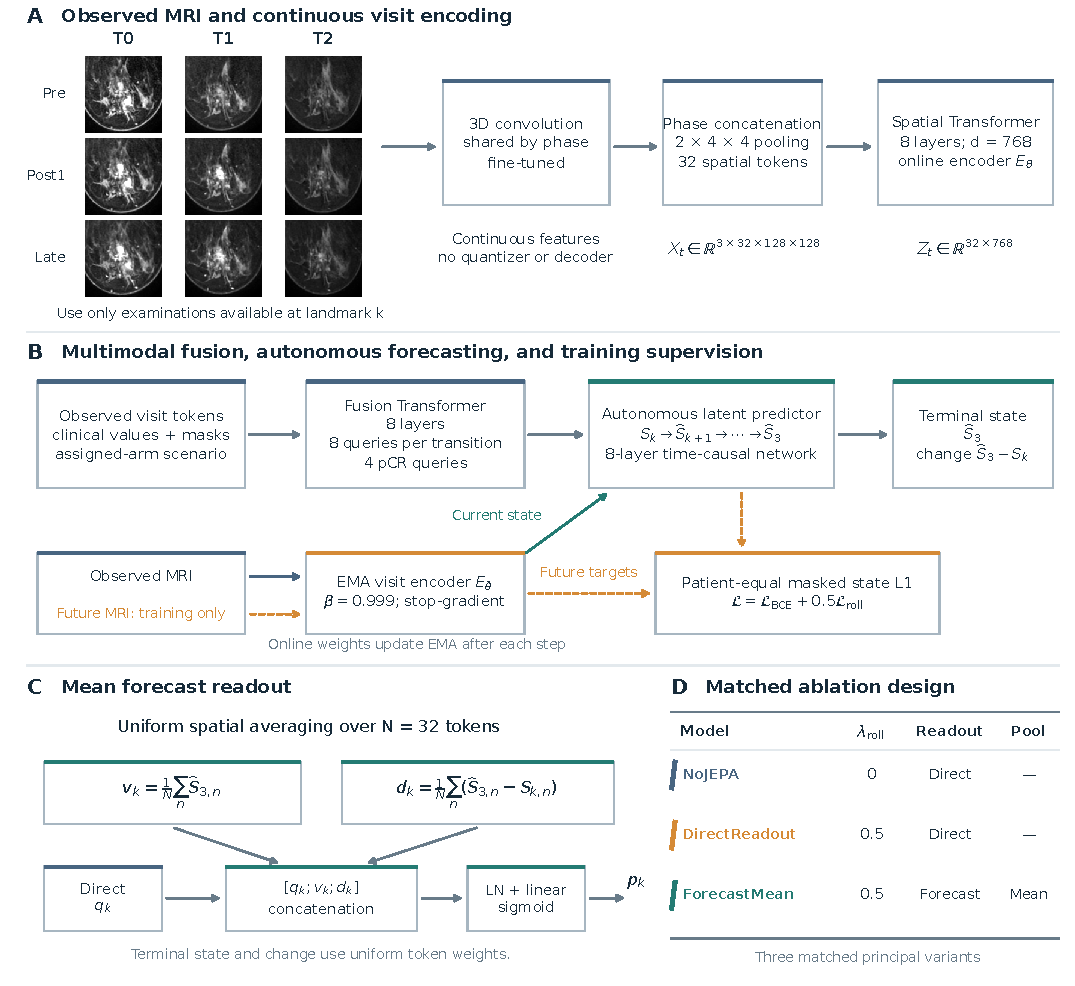
\includegraphics[width=\textwidth]{figures/framework.pdf}
\caption{Forecast-aware latent modeling and matched controls. (A) Real three-phase MRI crops from one development patient illustrate the same baseline-defined plane at T0, T1, and T2; the example and slice were selected without outcomes or pCR predictions. Only visits available at the prediction landmark are inputs. A shared continuous encoder and spatial Transformer produce visit tokens. (B) Clinical values, availability masks, and an assigned-arm scenario condition fusion and autonomous prediction to T3. The EMA encoder supplies the detached current state; available future MRI supplies training targets only. Dashed orange arrows denote training-target or loss paths. (C) Uniform spatial means pool the predicted terminal state and its change; these features are combined with direct pCR-query features. (D) The three primary variants separate removal of future-state supervision from the complete mean forecast readout. One fold model is illustrated. Within each of seeds 42, 44, 71, and 2026, evaluation averages five fold probabilities per patient before computing metrics; reported performance then averages the four seed metrics, without ensembling probabilities across seeds. MRI tiles are illustrative crops, not generated images, segmentation ground truth, or attention maps.}
\label{fig:framework}
\end{figure*}


\subsection{Longitudinal prediction problem}
\label{sec:problem}
We consider prediction of pathological complete response (pCR) from a patient's available magnetic resonance imaging (MRI) history during neoadjuvant treatment. Canonical examination stages are indexed by $t\in\{0,1,2,3\}$. At a prediction landmark $k\in\{0,1,2\}$, the model receives only examinations acquired and available by that landmark. Let $X_t\in\mathbb{R}^{3\times32\times128\times128}$ denote the processed examination at stage $t$, and let $o_t^{(k)}$ indicate whether this examination is available in the observed prefix. Missing examinations retain their canonical stage rather than shifting later examinations forward. The three channels contain the pre-contrast acquisition, the first post-contrast acquisition, and a metadata-selected late post-contrast acquisition, respectively. The late acquisition is not assumed to have the same acquisition index for all examinations.

The observed information is
\begin{equation}
 \mathcal{H}_k=\bigl\{(X_t,t):o_t^{(k)}=1\bigr\}\cup
 \bigl\{c_k,m_k,a_k,\tau_k\bigr\},
\end{equation}
where $c_k\in\mathbb{R}^{4}$ contains the available clinical variables, $m_k$ their availability indicators, $a_k$ the available assigned treatment-arm category, and $\tau_k$ its declared availability stage. The clinical variables are age at screening, hormone-receptor positivity, HER2 positivity, and a binary MammaPrint variable. Age is standardized using the current training partition; binary variables retain their original coding. Unavailable values are set to zero after standardization and accompanied by an explicit mask. The clinical token embeds the concatenated values and masks. Treatment conditioning uses 13 released arm categories and an additional unknown category. In this retrospective experiment, assigned arm and available baseline clinical variables are assumed to be known at T0. This is an assigned-arm scenario; the categorical input does not specify actual doses, treatment intervals, or treatment changes, and it does not support a causal interpretation.

The output is $p_k=\Pr(y=1\mid\mathcal{H}_k)$, where $y\in\{0,1\}$ is the final pCR label. Future MRI is stored separately as training supervision and is excluded from the prediction input. T3 can provide a future representation target during training, but is never a prediction landmark in the reported T0--T2 protocol.

\subsection{Continuous MRI encoding and multimodal fusion}
\label{sec:encoding}
Each observed examination is encoded independently by an online visit encoder $E_{\theta}$. Its convolutional front end shares the same single-channel weights across the three acquisition phases. Two stride-two three-dimensional convolutional stages, residual blocks, and group normalization produce 64 continuous feature channels per phase at one-quarter input resolution along each spatial axis. The three phase-specific feature maps are concatenated, adaptively averaged to a $2\times4\times4$ grid, and projected to a latent width of $d=768$. This gives $N=32$ spatial tokens per examination. Learned spatial positional embeddings and an eight-layer spatial Transformer then produce the visit representation $Z_t=E_{\theta}(X_t)\in\mathbb{R}^{N\times d}$.

The convolutional front end is initialized from the same pre-existing VQ-GAN-style codec checkpoint for all compared models and is fine-tuned. Here, the model uses continuous features from the codec encoder before its compression projection. It does not use discrete codebook assignments, a quantization objective, a decoder, or adversarial learning during downstream pCR training. \todo{Document the original codec pretraining dataset, patient-level overlap with the present partitions, checkpoint provenance, and applicable redistribution terms.}

Stage embeddings distinguish examination times. Observed image tokens, one clinical token, and one treatment-arm token form the multimodal context. An eight-layer fusion Transformer additionally receives eight learned transition-query tokens for each of the three canonical transitions and four pCR-query tokens. Transition-query slots are retained at every landmark, independently of which future targets happen to be available. Their conditioning is derived entirely from the observed prefix. Context tokens interact bidirectionally; appended transition and pCR queries use a causal attention mask and can attend to the context and preceding query positions. Padding masks remove unobserved image tokens. This produces transition features $A_{j+1}^{(k)}\in\mathbb{R}^{8\times d}$ for transitions $j\rightarrow j+1$, and pCR-query features $Q_k\in\mathbb{R}^{4\times d}$.

All spatial, fusion, and prediction Transformers use pre-normalization blocks, GELU feed-forward layers of width 3072, and dropout 0.3, following the attention-based architecture of \citet{vaswani2017}. Attention has 16 heads with 64 channels per head: its internal width is therefore 1024, followed by projection back to the 768-dimensional residual stream. The clinical and treatment tokens condition forecasting through the shared fusion network rather than through a separately supplied future treatment trajectory.

\subsection{EMA target states and autonomous forecasting}
\label{sec:forecasting}
A target visit encoder $E_{\bar\theta}$ is initialized as a copy of the online encoder and updated after each optimizer step by exponential moving average (EMA):
\begin{equation}
 \bar\theta\leftarrow\beta\bar\theta+(1-\beta)\theta,
 \qquad \beta=0.999.
\end{equation}
The target encoder remains in evaluation mode and receives no gradients. It defines a common representation space for the observed initial state and available future targets,
\begin{equation}
 S_t=\operatorname{stopgrad}\!\left(E_{\bar\theta}(X_t)\right)
 \in\mathbb{R}^{N\times d}.
\end{equation}
Encoding a future target in this branch supplies a loss target only; it does not make that examination available to the forecasting or classification input.

The predictor starts from the latest actually observed state in $\mathcal{H}_k$ and recursively advances to T3. For the reported landmarks, this initial state is $S_k$. At each future transition, it uses the corresponding transition features and its previously generated states. A history input additionally embeds the difference between a source state and its latest available predecessor, with a separate indicator for whether a predecessor exists. Observed history is used where available; after the landmark, the history is extended using model predictions. Thus, a missing future examination removes supervision at that time but does not interrupt the simulated transition sequence.

The prediction network is an eight-layer time-causal Transformer. Each transition block contains its eight transition tokens and 32 spatial source-state tokens, together with learned spatial and temporal embeddings. Tokens can interact within a block; attention between transition blocks is directed from earlier to later blocks. A learned root token remains available when some blocks are masked. The network predicts a residual state increment,
\begin{equation}
 \widehat S_{j+1}=\widetilde S_j+
 G_{\phi,j}\!\left(\widetilde S_{k:j},A_{k+1:j+1}^{(k)},D_{k:j}\right),
 \qquad j=k,\ldots,2,
\end{equation}
where $\widetilde S_k=S_k$, subsequent $\widetilde S_j$ are generated states, and $D_{k:j}$ denotes the available predecessor differences and validity indicators. The residual output projection is initialized to zero, so prediction initially preserves the source state. The transition features summarize the complete legal prefix even when only a subset of previous state differences is available to a particular prediction block.

Forecasts are generated autonomously during training and inference. A true future state never replaces a predicted predecessor. The classifier likewise uses this autonomous trajectory. The configuration includes no teacher-forced next-state loss in these experiments. EMA encoding of real future examinations is used exclusively to evaluate representation error against available targets.

\subsection{Prediction-conditioned pCR readout}
\label{sec:readout}
The full model, \fullmodel{}, combines a direct summary of the observed prefix with spatial arithmetic means of the predicted terminal state and its change from the current state. First, the four pCR-query features are averaged to obtain $q_k=\frac14\sum_{r=1}^{4}Q_{k,r}$. For spatial token $n$, the forecast change is $\Delta S_{k,n}=\widehat S_{3,n}-S_{k,n}$. The two forecast summaries are
\begin{equation}
 v_k=\frac{1}{N}\sum_{n=1}^{N}\widehat S_{3,n},
 \qquad
 d_k=\frac{1}{N}\sum_{n=1}^{N}\Delta S_{k,n}.
\end{equation}
All $N=32$ transformed spatial tokens receive the same pooling weight. The final prediction is
\begin{equation}
 p_k=\sigma\!\left(b+u^{\mathsf T}
 \operatorname{LN}\!\left([q_k;v_k;d_k]\right)\right).
\end{equation}
There is no learned spatial weighting in this classifier readout. The shared spatial, fusion, and forecasting Transformers retain their self-attention layers, so mean readout does not imply an attention-free network. Classification gradients propagate through the generated terminal state, predictor, and transition-conditioning pathway. The observed EMA reference state remains detached. Spatially transformed latent features are not validated anatomical localizations or tumor segmentations.

For \direct{}, pCR is instead predicted directly from $q_k$ using a layer-normalized linear head. Its future-state predictor is trained as an auxiliary task, but generated states are not explicit inputs to the pCR head. The direct head has input width $d$, whereas the full readout has width $3d$. Their comparison therefore evaluates the complete forecast-conditioned pathway, jointly changing access to predicted state and change features and classifier input width. It does not isolate the value of any single forecast feature.

\subsection{Training objective and matched ablations}
\label{sec:objective}
Let $\mathcal{B}_{y}$ be the labeled patients in a training batch, and let $m_{i,t}^{\mathrm{future}}$ indicate an actually available future target for patient $i$ after its sampled landmark. The pCR objective is unweighted binary cross-entropy,
\begin{equation}
 \mathcal{L}_{\mathrm{pCR}}=
 -\frac{1}{|\mathcal{B}_{y}|}\sum_{i\in\mathcal{B}_{y}}
 \left[y_i\log p_i+(1-y_i)\log(1-p_i)\right].
\end{equation}
Define $M_i=\sum_t m_{i,t}^{\mathrm{future}}$ and $\mathcal{B}_{+}=\{i:M_i>0\}$. Autonomous representation supervision is patient-equal:
\begin{equation}
 \mathcal{L}_{\mathrm{roll}}=
 \frac{1}{|\mathcal{B}_{+}|}\sum_{i\in\mathcal{B}_{+}}
 \frac{1}{M_i}\sum_t m_{i,t}^{\mathrm{future}}
 \frac{\|\widehat S_{i,t}-S_{i,t}\|_1}{Nd}.
\end{equation}
If a batch contains no future targets, this term is zero. Each available future examination has equal weight within a patient; the loss uses no horizon discount, lesion weighting, or fabricated target for a missing visit. Patients without future MRI still contribute pCR supervision.

The full model and \direct{} minimize
\begin{equation}
 \mathcal{L}=\mathcal{L}_{\mathrm{pCR}}+0.5\mathcal{L}_{\mathrm{roll}}.
\end{equation}
\nojepa{} uses the direct pCR head with $\mathcal{L}=\mathcal{L}_{\mathrm{pCR}}$. This historical control name denotes removal of future-state auxiliary supervision, rather than removal of every transition-related module: it retains the shared fusion architecture and transition-query slots. Consequently, \direct{} versus \nojepa{} isolates the added autonomous representation objective under the same direct readout, whereas \fullmodel{} versus \direct{} assesses the added forecast-conditioned classification pathway. The latter comparison changes both forecast-feature access and classifier input width.

All three models omit teacher-forced JEPA, image reconstruction, flow-matching, and variance-regularization losses. In particular, the future objective reported here is autonomous state prediction, despite the JEPA-related implementation lineage. During training, patients are shuffled once per epoch and one actual available T0--T2 landmark is sampled uniformly for each patient. This balances patient contributions without treating a patient with more visits as several independently sampled patients. The same clinical endpoint supervises each sampled prefix; validation assesses all available eligible prefixes using patient-equal weighting.

\section{Dataset and preprocessing}
\label{sec:data}

\subsection{Cohort construction and clinical variables}
We retrospectively analysed longitudinal breast dynamic contrast-enhanced MRI
(DCE-MRI) from the public I-SPY2 and ACRIN-6698 imaging
resources~\cite{tciaispy2_2022,tciaacrin6698_2021}. Source imaging identifiers
were linked to research identifiers using the accompanying official identity
mapping, and outcomes and baseline clinical variables were obtained from the
official I-SPY2 Imaging Cohort~1 clinical spreadsheet. The final cohort
comprised 976 patients with 3,641 usable examinations. Native imaging
identifiers belonged to the ISPY2 and ACRIN-6698 namespaces for 712 and 264
patients, respectively; these identifiers were mapped to the same clinical
release and do not define independent development and external validation
cohorts. The official collection pages identify the source imaging and clinical
release as CC BY 4.0. \todo{Confirm terms for redistributing derived assets and
document the applicable ethics approval or waiver and original consent arrangements.}

Eligibility required an actual baseline examination, an available binary pCR
label, usable baseline registered image assets, and a nonempty baseline
localisation produced by the existing MAMA-MIA segmentation workflow. Of 980
clinically matched source candidates, three lacked a baseline examination and
one had an empty or unavailable predicted baseline localisation. Their
exclusion yielded 976 patients and 3,642 candidate examinations. One
post-treatment examination was subsequently marked unavailable because its
saved within-examination phase transforms displaced the postcontrast images
outside the prescribed baseline crop. The patient's earlier examinations were
retained, leaving 3,641 usable examinations. Missing follow-up examinations did
not cause patient exclusion. No additional admission thresholds based on
normalised cross-correlation, field-of-view ratios, functional tumour volume,
or the availability of an accepted adjacent longitudinal pair were applied.

The endpoint was the released binary pCR field: 313 patients were labelled
positive and 663 negative. \todo{Verify and state the release-specific
pathological definition of pCR, including breast and nodal criteria and the
handling of in-situ disease; do not infer this definition from the binary
column alone.} Baseline covariates were age at screening, hormone-receptor
(HR) status, HER2 status, and the released binary MammaPrint indicator. Age was
available for 973 patients; all three binary covariates were available for the
entire cohort. The official assigned treatment arm, represented by 13
categories, was also supplied to the model. The current experiments use an
\emph{assigned-arm scenario}: the assigned arm and available baseline
covariates are assumed known at baseline. The spreadsheet does not establish
prospective allocation timestamps, doses, cycle-level exposure, or interval
treatment schedules, and the model does not reconstruct these quantities.

\begin{table*}[t]
\centering
\caption{Characteristics of the analysed cohort. Development statistics count
each of the 801 development patients once, rather than pooling overlapping
training folds. Age is reported as mean $\pm$ sample standard deviation among
patients with observed age; other entries are counts.}
\label{tab:cohort}
\small
\begin{tabular}{lrrr}
\toprule
Characteristic & All & Development & Holdout \\
\midrule
Patients & 976 & 801 & 175 \\
pCR positive & 313 & 257 & 56 \\
pCR negative & 663 & 544 & 119 \\
Age (years) & $48.7\pm10.5$ & $48.7\pm10.6$ & $48.9\pm10.2$ \\
Missing age & 3 & 3 & 0 \\
HR positive & 533 & 434 & 99 \\
HER2 positive & 240 & 195 & 45 \\
Available T0 & 976 & 801 & 175 \\
Available T1 & 935 & 760 & 175 \\
Available T2 & 875 & 700 & 175 \\
Available T3 & 855 & 692 & 163 \\
\bottomrule
\end{tabular}
\end{table*}

Examinations were indexed by the canonical study stages T0--T3 rather than
continuous elapsed time. Availability at these stages was 976, 935, 875, and
855 patients, respectively (Table~\ref{tab:cohort}); 803 patients had all four
examinations and 861 had T0--T2. The nominal source protocol acquired T0 before
randomization, T1 after three weeks of the first regimen (paclitaxel with or
without an experimental agent), T2 between paclitaxel and anthracycline
regimens, and T3 after four cycles of anthracycline treatment and before
surgery~\citep{tciaispy2_2022}. Because T0 MRI preceded randomization, supplying
the eventual assigned arm at T0 is a retrospective conditional scenario,
rather than a prospectively available predictor before treatment allocation.
The source protocol used 1.5 or 3.0 Tesla scanners with dedicated breast coils
and required the same scanner configuration within a patient. These are
nominal protocol specifications, not a patient-level audit of timing or
scanner compliance. Twenty-three patients had T0 only and remained
eligible for pCR supervision. Their unavailable future MRI targets were
masked, and no synthetic follow-up images were substituted. Model inputs and
evaluation landmarks were restricted to T0, T1, and T2; a real T3 examination,
when available in the training partition, could provide a future-state target.
\todo{Report the actual examination intervals, acquisition centres, scanner
distribution, and sequence-parameter ranges for the final analysed cohort.}

\subsection{Patient partitioning and evaluation scope}
The cohort was divided into 801 development patients and a fixed internal
holdout of 175 patients, including 56 pCR-positive patients. All holdout
patients had actual T0, T1, and T2 examinations, allowing matched longitudinal
evaluation; 163 also had T3. The holdout retained 139 patients with complete
T0--T2 observations from the historical benchmark and added 36 eligible
patients. Additional patients were selected using outcome quotas and a fixed
baseline-clinical distribution balancing rule with split seed 2026, without
using model predictions or performance. This fixed cohort-construction seed
is distinct from the training-seed comparison: the split is unchanged for
training seeds 42, 44, 71, and 2026. Development folds were stratified by
pCR and examination-availability pattern; rare joint strata were combined
within the same pCR class. Each development patient appeared in validation
exactly once across the five folds. Fold~1 contained 640 training and 161
validation patients; the remaining folds each contained 641 training and 160
validation patients. Training, validation, and holdout identities were
disjoint within each fold, and the same holdout was used for every fold
model at each training seed.

This partition is an internal downstream benchmark. In particular, 29 of the
36 added holdout patients had belonged to the development population of an
earlier experiment, so earlier trained models cannot be treated as held out
on the entire new set. The present downstream models were trained using the
new fold definitions. Patient independence of the supplied codec and
segmentation pretraining checkpoints relative to the final holdout has not
yet been established; that provenance must be audited before stronger claims
of end-to-end independence. The complete-examination holdout eligibility also
restricts inference about patients with missing early follow-up examinations.

\subsection{Registration, fixed localisation, and normalisation}
Within each examination, postcontrast phases were registered to the
precontrast reference. Follow-up examinations were aligned to the patient's
T0 reference using the saved longitudinal transforms, retaining a rigid
fallback when the final deformable candidate was not usable. Baseline
localisation used the existing MAMA-MIA nnU-Net prediction on the native
first-postcontrast examination~\cite{mamamia2025}. The centre of the largest
26-connected predicted component defined a fixed baseline crop, which was
reused at every actual follow-up. Follow-up segmentation and follow-up-driven
recentering were not used.

Each examination was represented by three channels: the precontrast phase,
the first postcontrast phase, and the late phase explicitly specified in the
examination metadata. The late channel was not selected by assuming a fixed
phase number or taking the last available phase. Images were resampled to
$32\times128\times128$ voxels with spacing
$2.0\times0.7032\times0.7032\,\mathrm{mm}$ in the slice and two in-plane
dimensions, approximately covering $64\times90\times90\,\mathrm{mm}$.
Linear interpolation was used for MRI intensities and nearest-neighbour
interpolation for masks and acquisition support, with zero padding outside
the acquired field of view. The localisation mask determined the crop; it was
not a contemporaneous ground-truth tumour segmentation or a future
observation supplied to the classifier.

Native metadata, baseline mask headers, registered reference grids, and saved
transforms were maintained as matched versions. Explicit array-index
mappings, rather than placeholder NIfTI affines, defined sampling positions.
The exported arrays were checked for finite values, consistent coordinate
mapping, and numerical agreement after compressed storage and readback.
These checks establish data and geometry consistency but do not establish
anatomical registration or segmentation accuracy. The fixed crop partly
truncated the largest predicted baseline component for 85 patients; these
patients were retained and the limitation was recorded.

Raw cropped intensities were stored once and shared across folds. For each
fold, a single intensity mean and population standard deviation were fitted
to nonzero precontrast foreground voxels from every unique actual examination
of that fold's training patients. The same scalar transform was applied once
to the foreground of all three channels, stages, and partitions; background
and padding remained zero. Validation and holdout images were excluded from
fitting. Age normalisation was likewise fitted to observed training-patient
values; HR, HER2, and MammaPrint retained their official binary coding, with
missingness represented explicitly.

\section{Experimental design}
\label{sec:experiments}
\subsection{Development protocol and landmark evaluation}
The 801 development patients were partitioned into five patient-level folds. Fold 1 used 640 training and 161 validation patients; folds 2--5 each used 641 training and 160 validation patients. The same 175-patient holdout was evaluated by every fold model and every variant. Within each seed and variant, the five test evaluations are repeated evaluations of overlapping trained models on the same patients, rather than five independent test cohorts. Repeating training seeds also reuses this holdout. Patient identities were disjoint between training, validation, and holdout within the current split.

At each training epoch, a patient contributed one randomly selected available T0, T1, or T2 prefix. Only MRI observations available at or before the selected landmark were classifier inputs. Later observed visits, including T3, could supply latent targets for the auxiliary loss on training patients. Missing targets were masked. The 23 patients with only T0 remained eligible for pCR training but supplied no future-state loss. At evaluation, all three landmarks were evaluated for the 175 holdout patients, each of whom had T0, T1, and T2. T3 was not an evaluation landmark and was not used as observed input for these predictions.

\subsection{Model comparisons}
The principal comparison comprises \nojepa{}, \direct{}, and \fullmodel{}, all trained with seeds 42, 44, 71, and 2026 using the same five development folds. Within each variant and seed, the five fold-specific models form an equal-weight probability ensemble. Performance is summarized across the four seed-specific ensembles by an equal mean of their metric values. \nojepa{} uses direct pCR readout and a zero future-state loss weight. \direct{} uses the same direct readout with a future-state loss weight of 0.5. \fullmodel{} retains that auxiliary weight and concatenates direct pCR features, the spatial arithmetic mean of the predicted terminal state, and the spatial arithmetic mean of its change from the current state. All three models retain the shared image encoder, clinical inputs, assigned-arm encoding, fusion architecture, and training schedule.

The \direct{}--\nojepa{} contrast most directly tests adding future-state supervision. The \fullmodel{}--\direct{} contrast jointly changes access to forecast features and classifier input width; it does not isolate a single feature contribution. All manuscript-facing pCR results first average five fold probabilities separately for each seed, patient, and landmark, compute metrics within each seed, and average those metrics across the four seeds. Probabilities are not averaged across seeds. All three reported variants are principal comparisons.

\subsection{Implementation and optimization}
The network uses a model width of 768, eight layers in each of the spatial encoder, multimodal fusion module, and predictor, 16 attention heads with 64 dimensions per head, and feed-forward width 3,072. The 1,024-dimensional concatenated attention-head representation is projected back to the 768-dimensional residual stream. The spatial token grid is $2\times4\times4$. The configuration uses eight state queries, four pCR queries, dropout 0.3, and an EMA coefficient of 0.999. The pretrained convolutional encoder is fine-tuned jointly with the remaining network. Its training-patient provenance requires additional documentation, as discussed in Section~\ref{sec:limitations}.

We use AdamW \citep{adamw2019} with an initial base learning rate of $10^{-4}$ for both the encoder and the main network, weight decay 0.05, batch size 16, no gradient accumulation, and gradient-norm clipping at 1.0. Training uses BF16 mixed precision. A ten-epoch warm-up increases the learning rate from $10^{-5}$ to $10^{-4}$, followed by cosine decay to $10^{-6}$ at epoch 100. Training is capped at 200 epochs, with early stopping after 50 epochs without improvement. The best checkpoint is selected independently in each fold using validation patient-equal-prefix F1 at threshold 0.5. This is an F1 selection protocol, even though AUROC is a principal reporting measure. Deterministic execution was not enabled, so a fixed seed does not imply bitwise reproducibility across hardware or software changes.

\subsection{Metrics, aggregation, and patient-level uncertainty}
We report 14 complementary metrics: AUROC, non-interpolated average precision (AP), F1, accuracy, sensitivity, specificity, positive and negative predictive value (PPV/NPV), balanced accuracy, Matthews correlation coefficient (MCC), Youden index, negative log-likelihood (NLL), Brier score, and expected calibration error (ECE) with ten equal-width probability bins. Confusion-matrix counts are additionally retained. Thresholded primary metrics use 0.5. MCC and balanced accuracy help interpret performance under class imbalance~\citep{chicco2020mcc}; positive prevalence is $56/175=0.32$. No holdout threshold optimization or probability recalibration was performed.

Let $p_{isf\ell}$ be the probability from the model trained with seed $s\in\mathcal{S}=\{42,44,71,2026\}$ in fold $f$ for patient $i$ at landmark $\ell$. Within each variant, the reporting estimand is
\begin{equation}
\begin{aligned}
 \bar p_{is\ell}&=\frac{1}{5}\sum_{f=1}^{5}p_{isf\ell},\\
 M_{s\ell}&=M\bigl(\{y_i,\bar p_{is\ell}\}_{i=1}^{175}\bigr),\\
 M_{s,\mathrm{macro}}&=\frac{1}{3}\sum_{\ell=0}^{2}M_{s\ell},\\
 \widehat M_\ell&=\frac{1}{4}\sum_{s\in\mathcal{S}}M_{s\ell}.
\end{aligned}
\end{equation}
Macro and seed averaging commute for these metric summaries; neither operation is a probability average across time or seeds. Thresholded metrics apply 0.5 separately to each seed's five-model ensemble probabilities. Main performance tables report the mean and sample standard deviation of the four seed-specific metrics, using the sample-variance denominator of three. Macro standard deviations are computed from the four seed-specific Macro values, rather than averaging landmark standard deviations. This spread describes the four selected training realizations. It is not a standard error, a patient-level interval, or evidence for the distribution of all possible training seeds. The estimand is the average performance of four five-model predictors; it is not the performance of a single twenty-model probability ensemble or a single model trained on the full development cohort. Individual-fold metrics remain audit-only.

For conditional patient-level uncertainty, we draw 2,000 bootstrap samples of the 175 patients with replacement. Each draw is shared across every seed, variant, and landmark. Within a draw, we recompute metrics separately from each seed-specific ensemble, average landmark metrics for Macro, and average the four seed metrics. The 2.5th and 97.5th percentiles give unadjusted intervals for this seed-mean metric or paired difference. Seeds are held fixed and are not resampled. The intervals therefore exclude retraining, retrospective seed-set selection, model selection, and aggregation-policy uncertainty. The five folds, four seeds, and three repeated landmarks do not increase the independent patient count beyond 175.

ROC and precision--recall curves are computed separately within each seed-specific probability ensemble, interpolated onto common false-positive-rate and recall grids, respectively, and then averaged across seeds for display. The numerical AUROC and non-interpolated AP are computed within seeds before averaging; their means need not equal the area under the displayed mean curve. Pointwise bands use the shared patient resamples and retain seed averaging. Reliability diagrams form five equal-count rank groups of 35 patients separately within each seed and average their group summaries across seeds. These are descriptive summaries of several predictors, distinct from the ten equal-width bins used to calculate each seed's ECE.

\subsection{Exploratory paired significance checks}
We use approximate, two-sided, null-centered paired patient-bootstrap tests for all 14 metrics, including AUROC~\citep{davison1997}. The tested quantity is the difference in the metric averaged across the four fixed seed-specific predictors. We generate $B=99{,}999$ shared patient resamples with random-number seed 20261103. Every resample draws 175 patients with replacement and is shared across seeds, models, and landmarks. Metrics are recomputed within seeds and then equally averaged, preserving all pairing. No model is retrained, no seed is resampled, and no fold- or seed-level $t$ test is used.

Let $\Delta_b^*$ denote the seed-mean metric difference in resample $b$ and $\Delta_{\mathrm{obs}}$ its observed value. We estimate the two-sided $p$ value by
\begin{equation}
 p=\frac{1+\sum_{b=1}^{B}\mathbb{I}\bigl(|\Delta_b^*-\Delta_{\mathrm{obs}}|\geq|\Delta_{\mathrm{obs}}|\bigr)}{B+1}.
\end{equation}
Ties are included. The plus-one convention prevents Monte Carlo zero values, but does not make this bootstrap approximation finite-sample exact. Non-smooth statistics such as AP, F1, and binned ECE warrant particular caution.

The principal reporting family contains nine tests: the three pairwise comparisons among \nojepa{}, \direct{}, and \fullmodel{}, each for Macro AUROC, AP, and F1. The secondary family contains 69 tests: 27 landmark-specific AUROC/AP/F1 comparisons among the principal models; 33 comparisons of the other 11 Macro metrics; and nine T2--T0 AUROC/AP/F1 comparisons within the three principal models. Holm adjustment~\citep{holm1979} is applied separately within each family. The aggregate CSV additionally reports an all-78 Holm sensitivity analysis; separate-family adjustments do not control the familywise error rate over the union. We use $p_{\mathrm{Holm}}<0.05$, with $*$, $**$, and $***$ denoting adjusted values below 0.05, 0.01, and 0.001, respectively, and ns otherwise.

The 2,000-resample percentile intervals remain unadjusted and are not exact inversions of these tests. We compute $p$ values from the bootstrap differences rather than deriving them from whether an interval includes zero. The seed set, aggregation policy, testing procedure, and reporting families were selected retrospectively after results were available. All inference is exploratory and conditions on these fitted predictors; it does not measure uncertainty from retraining or retrospective selection. OOF-threshold, subgroup, decision-curve, and training-probe summaries receive no additional significance tests.



The T2 AUROC comparison of \fullmodel{} versus \nojepa{} had an all-78 adjusted value close to 0.05 relative to its Monte Carlo uncertainty. As a numerical sensitivity check, we repeat this same null-centered paired patient-bootstrap hypothesis with 999,999 resamples and independent random-number seed 20261104. Each resample recomputes T2 AUROC separately for all four seed-specific ensembles before averaging their differences. We recalculate Holm adjustment with only this $p$ value replaced and the other 77 held fixed. This is a separate numerical check; the uniformly generated 99,999-resample values and markers remain in the main tables.

\subsection{Operating-point and hypothetical decision analyses}
As a threshold sensitivity analysis, within each training seed, each development patient's out-of-fold (OOF) probability is supplied only by the fold model for which that patient was in validation. These patients also informed their fold-specific best-checkpoint selection, so the OOF scores are not a nested or independent calibration set. The disjoint validation predictions are concatenated separately for every seed at T0, T1, and T2, and Youden index is maximized on the resulting OOF scores, with the highest threshold resolving ties. The threshold is then applied to holdout ensemble probabilities. The OOF score for a development patient comes from one model, whereas the holdout score averages five models; their score distributions can differ. This analysis therefore examines threshold transfer and does not supply independent validation or calibration of the five-model ensemble. No holdout outcome selects a threshold. Bootstrap intervals hold the OOF-selected threshold fixed.

We additionally compute exploratory decision curves~\citep{vickers2006dca}. At risk threshold $q$, the generic positive action is applied when predicted pCR probability is at least $q$. Its mathematical net benefit is
\begin{equation}
 \mathrm{NB}(q)=\frac{\mathrm{TP}(q)}{n}
 -\frac{\mathrm{FP}(q)}{n}\frac{q}{1-q}.
\end{equation}
We calculate this separately from each seed's five-fold ensemble probabilities over thresholds 0.05--0.80, average the three landmark net benefits for Macro, and then average across the four seeds. Treat-all and treat-none are references. The calculation uses uncalibrated probabilities and does not validate a particular escalation, de-escalation, or other management action.

\subsection{Exploratory subgroup and mechanism analyses}
We examine released HR/HER2 combinations, age below or at least 50 years, native source namespace, and saved predicted-component crop coverage. Age 50 is an exploratory reporting cutpoint. Subgroup AUROC/AP are suppressed when fewer than ten patients or fewer than five outcomes in either class are available. Subgroup metrics are computed within each seed's five-fold ensemble and then averaged across seeds. Paired within-subgroup patient resampling preserves seed, model, and landmark pairing; single-class draws are omitted for AUROC intervals and valid-draw counts retained. Intervals are unadjusted, and no subgroup-interaction hypothesis is tested. Source namespaces share the same clinical release and are not independent external cohorts.

Mechanism analysis is restricted to archived fixed-training-probe diagnostics collected every five epochs. These probes sample up to 32 training patients and are not full validation or holdout forecast evaluations. Unlike the missing-target-masked training objective, the archived forecast diagnostic includes only continuous observed visit chains: the real landmark, target, and every intermediate canonical visit must be available. A gap excludes that landmark--target pair, and eligible-patient counts therefore vary by horizon. We report a descriptive common epoch 20 and common-epoch trajectories. Forecast skill is $1-\mathrm{L1}_{\mathrm{forecast}}/\mathrm{L1}_{\mathrm{copy}}$ within the same snapshot's EMA representation; the copy forecast holds the observed landmark state constant. This normalization avoids comparing raw latent errors between separately learned teacher coordinates. Predictor gradient norms from the pCR and weighted rollout objectives are descriptive checks of gradient routing, not independent statistical samples or clinical effects. These archived diagnostics are computed within each model's own EMA coordinates, averaged over the five folds within each seed, and then summarized across the four seeds. Only epochs with complete diagnostic coverage are used for common-epoch summaries. They do not ensemble latent states and should be distinguished from the probability-ensemble pCR evaluation.

\subsection{Scope of the selected four-seed analysis}
The overall-model choice of mean forecast readout and seeds 42, 44, 71, and 2026 were selected after holdout results from other model and seed combinations had been available. This is a retrospective change in the reporting model and seed set, not a prospectively specified analysis. Applying the same set, folds, and aggregation rule to every model preserves a matched comparison but does not remove selection bias. Four-seed standard deviations describe this selected subset; patient-bootstrap intervals and tests condition on its fitted predictors. A confirmatory study should lock training seeds, overall-model and checkpoint selection, aggregation, statistical comparisons, and operating-point policies before evaluating independent patients.

\section{Results}
\label{sec:results}
\subsection{Discrimination across four training seeds}
All 60 runs of the three principal models completed training and formal evaluation. Sixty evaluation receipts and 180 registered report identities were verified. Every seed-specific predictor averaged five fold probabilities for each of the same 175 holdout patients, including 56 positive outcomes. We then calculated metrics within each seed and averaged the metrics across seeds 42, 44, 71, and 2026. Table~\ref{tab:main} reports means with sample seed standard deviations; conditional patient intervals and paired tests are reported separately.
\begin{table*}[t]
\centering
\small
\caption{Performance on the fixed internal holdout (175 patients, 56 pCR positive). Entries are mean $\pm$ sample SD over seeds 42, 44, 71, and 2026. Within each seed, five fold probabilities are averaged per patient before metrics; no probabilities are averaged across seeds. Macro averages T0--T2 metrics within each seed. F1 uses threshold 0.5. Paired Macro differences and adjusted tests are in Table~\ref{tab:bootstrap}.}
\label{tab:main}
\begin{tabular}{llrrr}
\toprule
Model & Landmark & AUROC & AP & F1 \\
\midrule
NoJEPA & T0 & 0.7270 $\pm$ 0.0037 & 0.5898 $\pm$ 0.0092 & 0.5332 $\pm$ 0.0152 \\
NoJEPA & T1 & 0.7251 $\pm$ 0.0054 & 0.5911 $\pm$ 0.0093 & 0.5399 $\pm$ 0.0107 \\
NoJEPA & T2 & 0.7254 $\pm$ 0.0051 & 0.5907 $\pm$ 0.0076 & 0.5416 $\pm$ 0.0166 \\
NoJEPA & Macro & 0.7258 $\pm$ 0.0044 & 0.5905 $\pm$ 0.0086 & 0.5382 $\pm$ 0.0138 \\
DirectReadout & T0 & 0.7341 $\pm$ 0.0089 & 0.5932 $\pm$ 0.0091 & 0.5392 $\pm$ 0.0189 \\
DirectReadout & T1 & 0.7369 $\pm$ 0.0107 & 0.6010 $\pm$ 0.0145 & 0.5388 $\pm$ 0.0261 \\
DirectReadout & T2 & 0.7353 $\pm$ 0.0071 & 0.5975 $\pm$ 0.0123 & 0.5556 $\pm$ 0.0097 \\
DirectReadout & Macro & 0.7354 $\pm$ 0.0087 & 0.5972 $\pm$ 0.0107 & 0.5446 $\pm$ 0.0176 \\
ForecastMean & T0 & 0.7476 $\pm$ 0.0060 & 0.6162 $\pm$ 0.0159 & 0.5739 $\pm$ 0.0130 \\
ForecastMean & T1 & 0.7494 $\pm$ 0.0070 & 0.6205 $\pm$ 0.0138 & 0.5821 $\pm$ 0.0149 \\
ForecastMean & T2 & 0.7478 $\pm$ 0.0076 & 0.6225 $\pm$ 0.0123 & 0.5719 $\pm$ 0.0036 \\
ForecastMean & Macro & 0.7483 $\pm$ 0.0067 & 0.6197 $\pm$ 0.0137 & 0.5760 $\pm$ 0.0083 \\
\bottomrule
\end{tabular}
\end{table*}


\fullmodel{} had mean T0/T1/T2 AUROCs of 0.7476/0.7494/0.7478 and AP values of 0.6162/0.6205/0.6225 (Fig.~\ref{fig:discrimination}). Its Macro AUROC/AP/F1 was 0.7483/0.6197/0.5760, with sample seed standard deviations of 0.0067/0.0137/0.0083. Corresponding means were 0.7258/0.5905/0.5382 for \nojepa{} and 0.7354/0.5972/0.5446 for \direct{}. Forecast mean had the highest mean AUROC, AP, and F1 at every landmark among the three reported models. Its T2 F1 was 0.5719, compared with 0.5556 for \direct{} and 0.5416 for \nojepa{}. These are averages of metrics from four separately evaluated seed-specific ensembles, not metrics of a combined predictor.

\begin{figure*}[t]
\centering
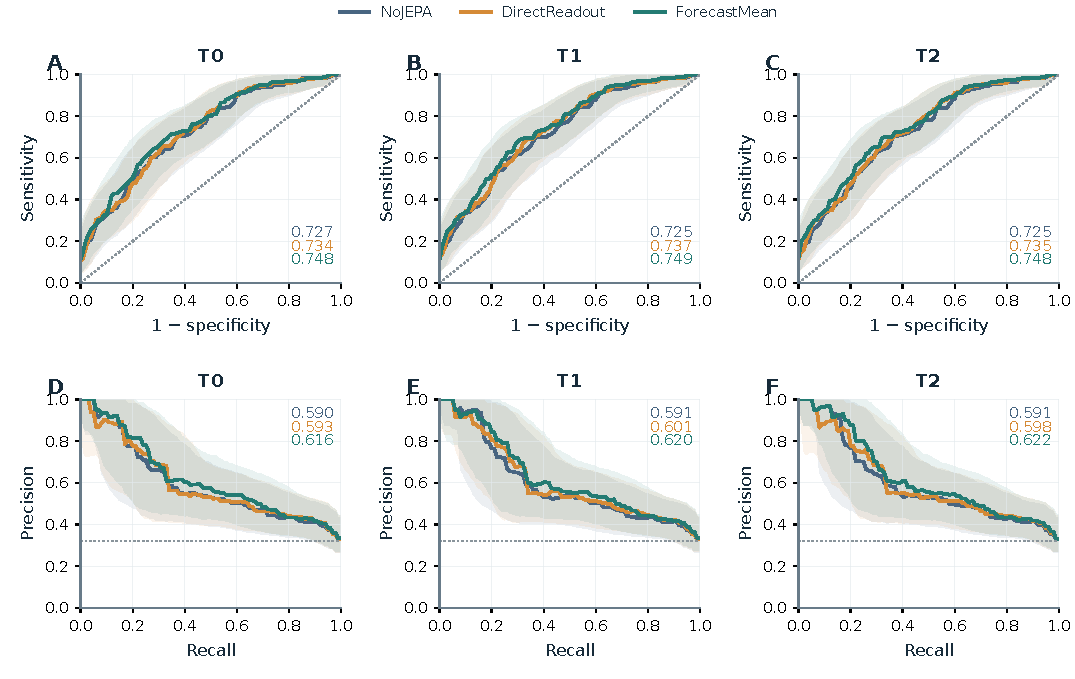
\includegraphics[width=\textwidth]{figures/discrimination.pdf}
\caption{Discrimination across seeds 42, 44, 71, and 2026. (A--C) Mean ROC curves; (D--F) mean precision--recall curves. Curves are computed from five-fold ensemble probabilities separately within each seed, interpolated on a common grid, and equally averaged across seeds. Shading gives pointwise conditional 95\% shared-patient-bootstrap intervals for the mean curve. Colored metric values are means of the directly computed seed-specific AUROC or non-interpolated AP; they need not equal the area under the displayed mean curve. The dotted PR reference is the 0.32 positive prevalence.}
\label{fig:discrimination}
\end{figure*}

Under direct readout, adding future-state supervision increased mean Macro AUROC/AP/F1 by +0.0096/+0.0067/+0.0063. Adding the complete mean forecast readout increased these means by a further +0.0129/+0.0225/+0.0314 relative to \direct{}. These means conceal variation among seeds. The direct-versus-\nojepa{} Macro AUROC comparison was negative at seed 2026 (0.7230 versus 0.7251). Forecast mean had lower AUROC than \direct{} at seed 42 (0.7407 versus 0.7428), despite higher AP and F1. Its Macro AUROC/AP/F1 at seed 71 was 0.7569/0.6394/0.5869; the corresponding direct-readout values were 0.7358/0.5825/0.5369. The full-versus-\nojepa{} Macro AUROC difference was positive at all four selected seeds. The supplementary seed tables retain each realization, including the unfavorable contrasts; the selected subset does not establish behavior across all possible seeds.


Paired patient intervals qualify the descriptive rankings (Fig.~\ref{fig:paired}). The mean Macro AUROC difference for \fullmodel{} versus \nojepa{} was +0.0225 [0.0106, 0.0347]. The corresponding \direct{}--\nojepa{} difference was +0.0096 [0.0002, 0.0193], and the \fullmodel{}--\direct{} difference was +0.0129 [0.0021, 0.0236]. The full-versus-\nojepa{} AP/F1 differences were +0.0292 [0.0078, 0.0508] and +0.0377 [0.0034, 0.0782]. Against \direct{}, they were +0.0225 [0.0043, 0.0411] and +0.0314 [0.0003, 0.0697]. These unadjusted intervals concern patient sampling conditional on the selected fitted predictors and are distinct from descriptive seed standard deviations or multiplicity-adjusted tests.

The full-versus-\nojepa{} Macro AUROC difference had approximate paired-bootstrap raw $p=0.00050$, nine-test Holm $p=0.00450$, and all-78 Holm $p=0.03850$. It was the only principal comparison meeting the family-adjusted 0.05 criterion. The corresponding AP and F1 comparisons had raw/within-family adjusted $p=0.01020/0.08160$ and 0.04513/0.22565, respectively. All three full-versus-direct Macro comparisons remained nonsignificant after principal-family adjustment: AUROC/AP/F1 adjusted values were 0.13699/0.13699/0.22565. The auxiliary-supervision AUROC comparison also did not pass adjustment (raw $p=0.04678$, adjusted 0.22565). Nonsignificance does not establish equivalence.

Within the secondary family, only the full-versus-\nojepa{} T1 and T2 AUROC differences met the adjusted criterion. T1 had a difference of +0.0243 [0.0117, 0.0372], raw $p=0.00036$, secondary-family Holm $p=0.02484$, and all-78 Holm $p=0.02808$. T2 had a difference of +0.0224 [0.0100, 0.0353], raw $p=0.00058$, secondary-family Holm $p=0.03944$, and all-78 Holm $p=0.04408$. The Macro, T1, and T2 AUROC contrasts were the only three comparisons meeting the all-78 criterion. They remain conditional on the retrospectively selected predictors and reporting policy.

The independent 999,999-resample T2 AUROC check yielded raw $p=0.000722$ with Monte Carlo standard error approximately 0.0000269. Replacing only this entry and holding the other 77 values fixed gave secondary-family Holm $p=0.049096$ and all-78 Holm $p=0.054872$. Thus the T2 all-78 decision crossed the 0.05 threshold relative to the uniform-table value 0.04408; it should not be interpreted as robust to numerical precision. Macro and T1 retain their original values in this sensitivity calculation, but their bootstrap simulations were not repeated. The main table continues to report the uniform 99,999-resample analysis.
\begin{table*}[t]
\centering
\small
\caption{Exploratory principal Macro comparisons. All metrics use approximate, null-centered paired patient-bootstrap tests with 99,999 shared resamples. Within each draw, metrics are computed for each seed then equally averaged. All $p$ values are two-sided. Holm$_9$ adjusts the nine entries here; Holm$_{78}$ is the sensitivity analysis over all 78 principal and secondary tests. Sig. refers to Holm$_9$. Direct and Mean abbreviate DirectReadout and ForecastMean. $^{*}p_{\mathrm{Holm}}<0.05$, $^{**}p_{\mathrm{Holm}}<0.01$, $^{***}p_{\mathrm{Holm}}<0.001$; ns, not significant after the stated correction. Intervals are unadjusted 95\% patient-bootstrap intervals (2,000 shared draws) and need not agree with adjusted test decisions. All analyses condition on the fixed, retrospectively selected seed42/44/71/2026 ensembles; seeds are not resampled.}
\label{tab:bootstrap}
\begin{tabular}{llrrrrc}
\toprule
Comparison & Metric & Difference [95\% CI] & $p$ & $p_{\mathrm{Holm},9}$ & $p_{\mathrm{Holm},78}$ & Sig. \\
\midrule
Direct -- NoJEPA & AUROC & +0.0096 [+0.0002, +0.0193] & 0.0468 & 0.2257 & 1.0000 & ns \\
Direct -- NoJEPA & AP & +0.0067 [-0.0055, +0.0203] & 0.3092 & 0.6185 & 1.0000 & ns \\
Direct -- NoJEPA & F1 & +0.0063 [-0.0098, +0.0216] & 0.4079 & 0.6185 & 1.0000 & ns \\
Mean -- NoJEPA & AUROC & +0.0225 [+0.0106, +0.0347] & 0.0005 & 0.0045 & 0.0385 & ** \\
Mean -- NoJEPA & AP & +0.0292 [+0.0078, +0.0508] & 0.0102 & 0.0816 & 0.7140 & ns \\
Mean -- NoJEPA & F1 & +0.0377 [+0.0034, +0.0782] & 0.0451 & 0.2257 & 1.0000 & ns \\
Mean -- Direct & AUROC & +0.0129 [+0.0021, +0.0236] & 0.0202 & 0.1370 & 1.0000 & ns \\
Mean -- Direct & AP & +0.0225 [+0.0043, +0.0411] & 0.0196 & 0.1370 & 1.0000 & ns \\
Mean -- Direct & F1 & +0.0314 [+0.0003, +0.0697] & 0.0730 & 0.2257 & 1.0000 & ns \\
\bottomrule
\end{tabular}
\end{table*}


\begin{figure*}[t]
\centering
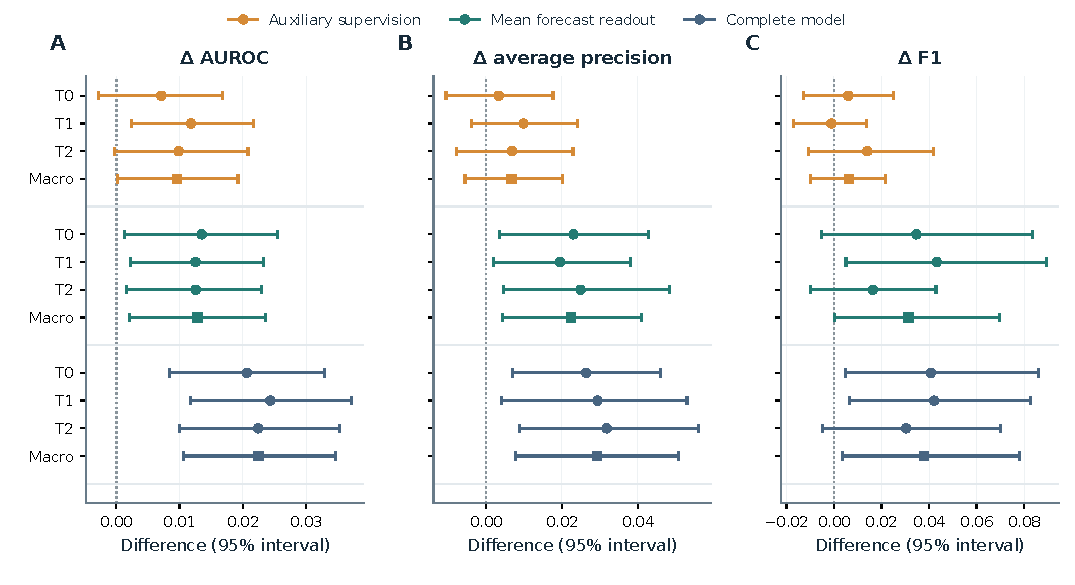
\includegraphics[width=\textwidth]{figures/paired_comparisons.pdf}
\caption{Paired seed-mean metric differences at T0, T1, T2, and Macro. Colors distinguish auxiliary supervision, additional forecast readout, and the complete-model contrast. Squares denote Macro estimates. Bars are unadjusted 95\% patient-bootstrap intervals. Every draw is shared across seeds, models, and landmarks; metrics are computed within seed before averaging. Adjusted tests appear in Tables~\ref{tab:bootstrap} and~\ref{tab:significance_landmarks}. Folds, seeds, and repeated landmarks do not create independent test cohorts.}
\label{fig:paired}
\end{figure*}

\subsection{Threshold behavior and class imbalance}
\begin{table*}[t]
\centering
\small
\caption{Operating characteristics at threshold 0.5. Entries average the four seed-specific fivefold probability-ensemble metrics; Macro first averages T0--T2 within each seed. The same 175 patients appear in every evaluation.}
\label{tab:extended_operating}
\begin{tabular}{llrrrrrr}
\toprule
Model & Landmark & Sens. & Spec. & PPV & NPV & BA & MCC \\
\midrule
NoJEPA & T0 & 0.580 & 0.721 & 0.496 & 0.786 & 0.650 & 0.291 \\
NoJEPA & T1 & 0.598 & 0.710 & 0.494 & 0.790 & 0.654 & 0.296 \\
NoJEPA & T2 & 0.603 & 0.708 & 0.493 & 0.792 & 0.655 & 0.297 \\
NoJEPA & Macro & 0.594 & 0.713 & 0.494 & 0.789 & 0.653 & 0.295 \\
\midrule
DirectReadout & T0 & 0.576 & 0.737 & 0.510 & 0.787 & 0.657 & 0.305 \\
DirectReadout & T1 & 0.580 & 0.731 & 0.505 & 0.788 & 0.656 & 0.302 \\
DirectReadout & T2 & 0.634 & 0.695 & 0.495 & 0.802 & 0.665 & 0.313 \\
DirectReadout & Macro & 0.597 & 0.721 & 0.503 & 0.792 & 0.659 & 0.307 \\
\midrule
ForecastMean & T0 & 0.674 & 0.683 & 0.500 & 0.817 & 0.678 & 0.336 \\
ForecastMean & T1 & 0.679 & 0.693 & 0.510 & 0.821 & 0.686 & 0.351 \\
ForecastMean & T2 & 0.683 & 0.668 & 0.492 & 0.818 & 0.676 & 0.330 \\
ForecastMean & Macro & 0.679 & 0.681 & 0.501 & 0.819 & 0.680 & 0.339 \\
\bottomrule
\end{tabular}
\end{table*}

At threshold 0.5, mean Macro sensitivity/NPV was 0.6786/0.8186 for \fullmodel{}, compared with 0.5967/0.7924 for \direct{}. These increases accompanied lower specificity (0.6814 versus 0.7213) and slightly lower PPV (0.5008 versus 0.5033). The paired mean sensitivity difference was +0.0818 [0.0404, 0.1327], while the specificity difference was $-0.0399$ [$-0.0663$, $-0.0165$]. Relative to \nojepa{}, sensitivity increased by +0.0848 [0.0396, 0.1398] and specificity decreased by $-0.0315$ [$-0.0603$, $-0.0057$]. These unadjusted intervals describe an operating trade-off. Against \direct{}, raw/secondary-family adjusted $p$ values were 0.00127/0.08509 for sensitivity and 0.00191/0.12415 for specificity. No operating or probability-quality comparison met the secondary-family adjusted criterion.



The full model's seed-mean true-positive counts at T0/T1/T2 were 37.75/38.00/38.25, with false-positive counts 37.75/36.50/39.50. These are averages of integer counts from four correlated predictors, not fractional patients or a single combined confusion matrix. Mean F1 increased from 0.5739 at T0 to 0.5821 at T1, then decreased to 0.5719 at T2. The additional T2 positive predictions included more false positives, illustrating why further observations need not improve a fixed-threshold decision rule.

\fullmodel{} had the highest mean Macro balanced accuracy (0.6800) and MCC (0.3391), compared with 0.6590/0.3066 for \direct{} and 0.6533/0.2947 for \nojepa{}. Accuracy was 0.6814 for \direct{}, 0.6805 for forecast mean, and 0.6748 for \nojepa{}. The first two means were only slightly above the all-negative reference of 0.68. Accuracy, ranking, and class-specific errors therefore give different descriptive orderings.

OOF-selected Youden thresholds changed mean holdout Macro F1 from 0.5382 to 0.5418 for \nojepa{}, 0.5446 to 0.5420 for \direct{}, and 0.5760 to 0.5743 for \fullmodel{} (Table~\ref{tab:extended_threshold}). Thus the alternative threshold produced a small increase for \nojepa{} and decreases for the other models. These results concern transfer of thresholds fitted on single-model OOF scores to within-seed five-model ensemble scores; they neither optimize a holdout threshold nor establish independent ensemble calibration.

\subsection{Longitudinal information and probability quality}
The paired seed-mean T2--T0 AUROC change was +0.0002 [$-0.0054$, 0.0061] for \fullmodel{}, $-0.0016$ [$-0.0064$, 0.0029] for \nojepa{}, and +0.0011 [$-0.0034$, 0.0057] for \direct{}. The full model's corresponding AP change was +0.0062 [$-0.0063$, 0.0194] and F1 change $-0.0020$ [$-0.0125$, 0.0095]. All these longitudinal intervals included zero. Forecast mean's AUROC was highest at T1, whereas mean AP increased across landmarks; neither pattern establishes a confirmed benefit from an additional visit. Fig.~\ref{fig:scorechanges} shows outcome-conditioned distributions of changes in seed-specific ensemble probabilities.

\begin{table*}[t]
\centering
\small
\caption{Probability quality: four-seed mean $\pm$ sample SD of Macro metrics. Each seed has its own fivefold probability ensemble. Lower is better; ECE uses ten equal-width bins.}
\label{tab:calibration}
\begin{tabular}{lrrr}
\toprule
Model & NLL & Brier & ECE \\
\midrule
NoJEPA & 0.5812 $\pm$ 0.0081 & 0.1996 $\pm$ 0.0036 & 0.1157 $\pm$ 0.0196 \\
DirectReadout & 0.5771 $\pm$ 0.0104 & 0.1979 $\pm$ 0.0045 & 0.1207 $\pm$ 0.0204 \\
ForecastMean & 0.5829 $\pm$ 0.0118 & 0.2002 $\pm$ 0.0054 & 0.1405 $\pm$ 0.0178 \\
\bottomrule
\end{tabular}
\end{table*}

Mean Macro NLL/Brier/ECE was 0.5829/0.2002/0.1405 for \fullmodel{}, compared with 0.5771/0.1979/0.1207 for \direct{} and 0.5812/0.1996/0.1157 for \nojepa{}. Forecast mean had worse point estimates of all three probability-quality metrics than both direct-readout controls. The higher discrimination means therefore did not translate into better probability-quality means. All 14 Macro metrics and their conditional patient intervals appear in Table~\ref{tab:extended_macro}.

\begin{figure*}[t]
\centering
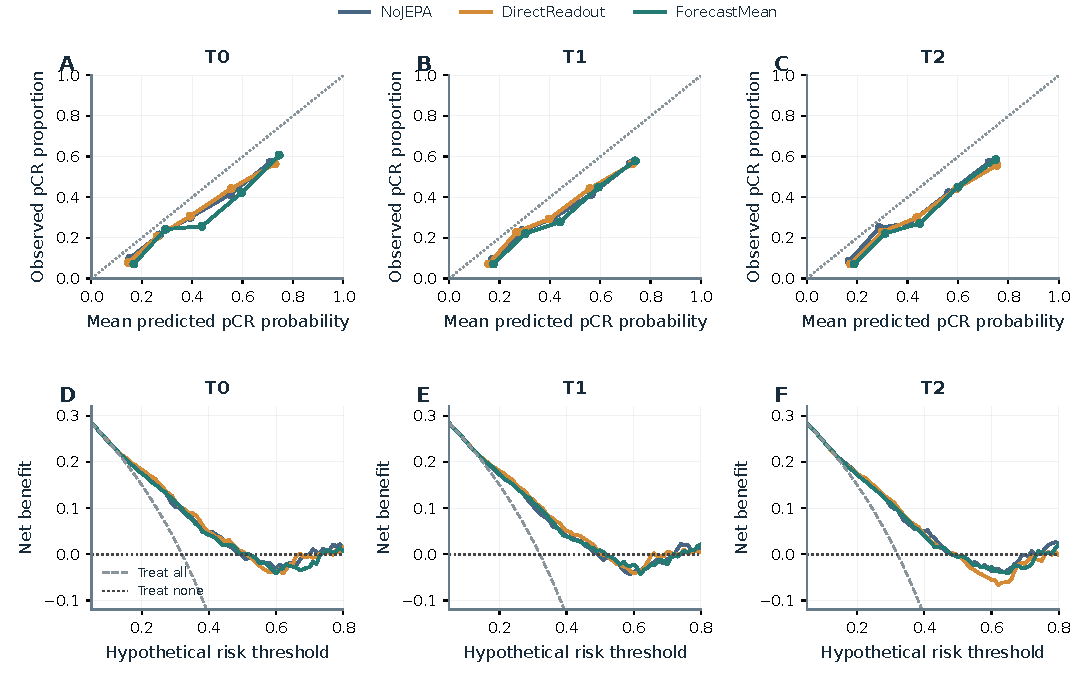
\includegraphics[width=\textwidth]{figures/calibration_utility.pdf}
\caption{Probability quality and hypothetical decision utility across four seeds. (A--C) Reliability summaries first form five equal-count probability-rank groups of 35 patients within each seed-specific five-fold ensemble and then average the group summaries across seeds. They differ from the ten equal-width bins used for ECE. (D--F) Net-benefit curves are computed separately within seeds and then averaged, with treat-all and treat-none references. Scores are not recalibrated. No clinical escalation or de-escalation strategy is validated.}
\label{fig:calutility}
\end{figure*}

\subsection{Hypothetical net benefit}
Decision curves did not preserve the discrimination ranking across thresholds. At a hypothetical threshold of 0.30, mean Macro net benefit was 0.1169 for \direct{} and 0.1118 for \fullmodel{}. At 0.50, it was $-0.0052$ for \nojepa{}, +0.0014 for \direct{}, and +0.0005 for \fullmodel{}. At 0.70, forecast mean had lower net benefit ($-0.0267$) than direct readout ($-0.0067$). These values average seed-specific decision curves, use uncalibrated probabilities, and assume a generic positive action. They do not establish an acceptable clinical threshold or validate a management pathway.

\subsection{Exploratory biological and acquisition-related subgroups}
The four HR/HER2 groups had positive seed-mean Macro AUROC differences between \fullmodel{} and \nojepa{} (Fig.~\ref{fig:subgroups}; Table~\ref{tab:subgroups}). The HR-positive/HER2-negative group had a difference of +0.0385 [0.0089, 0.0743] among 68 patients, including 11 positive outcomes. Other differences were +0.0143 [$-0.0349$, 0.0629] in HR-positive/HER2-positive patients (31, 12 positive), +0.0272 [$-0.0272$, 0.1136] in HR-negative/HER2-positive patients (14, 7 positive), and +0.0380 [0.0083, 0.0705] in HR-negative/HER2-negative patients (62, 26 positive). The first and fourth groups' unadjusted intervals excluded zero. These exploratory intervals do not establish a multiplicity-adjusted subtype benefit or an interaction.

In the HR-positive/HER2-negative group, forecast mean's mean Macro sensitivity/specificity was 0.1515/0.9620, compared with 0.1061/0.9868 for \nojepa{}. Thus low sensitivity at threshold 0.5 persisted despite the positive AUROC difference. \direct{} had sensitivity/specificity 0.0985/0.9912. Mean Macro AUROC was 0.7197 for forecast mean, 0.7064 for \direct{}, and 0.6812 for \nojepa{}. Age-group summaries remain exploratory and do not support an age-interaction conclusion. Source namespaces share one clinical release and do not constitute external validation. The partially clipped baseline-component group contained only 11 patients and one positive outcome; its AUROC and AP were suppressed under the minimum-outcome rule.

\begin{figure*}[t]
\centering
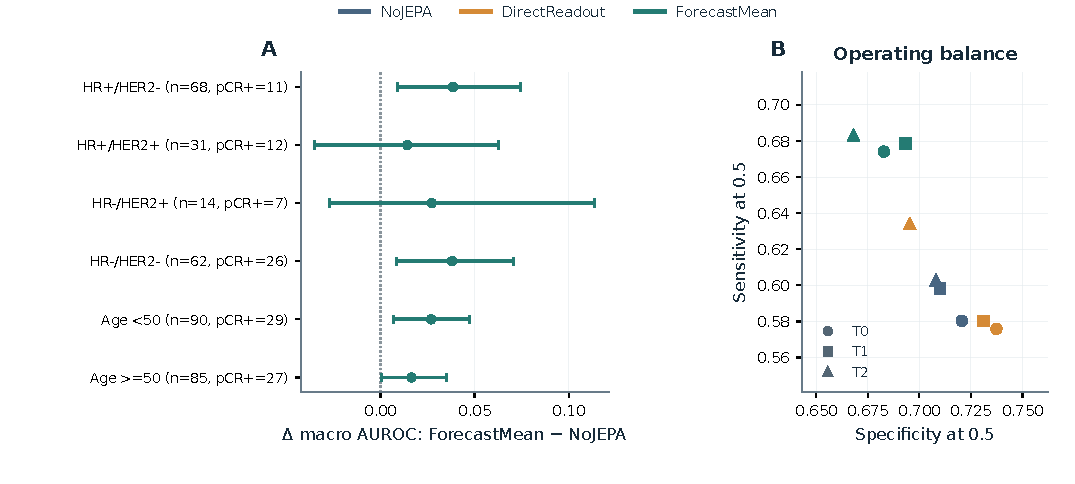
\includegraphics[width=\textwidth]{figures/subgroup_operating.pdf}
\caption{Exploratory subgroup and operating-point summaries, with metrics computed within seed and then equally averaged across seeds 42, 44, 71, and 2026. (A) Macro AUROC differences between ForecastMean and NoJEPA within HR/HER2 and age groups, with patient counts, positive outcomes, and unadjusted shared-patient intervals. No subgroup-interaction claim is made. (B) Mean specificity and sensitivity at threshold 0.5 across landmarks; colors identify models and markers identify landmarks.}
\label{fig:subgroups}
\end{figure*}

\subsection{Archived forecast and gradient diagnostics}
Archived fixed-training-probe diagnostics describe individual models separately from the pCR holdout analysis (Fig.~\ref{fig:mechanism}). At common epoch 20, mean copy-normalized forecast skills for \direct{} were +0.0129, +0.0621, and +0.1635 at one-, two-, and three-step horizons. Corresponding values for \fullmodel{} were $-0.0469$, $-0.0479$, and +0.0283 (Table~\ref{tab:worldprobe}). Statistics were normalized within each snapshot's EMA coordinates, averaged across five folds within seed, and then averaged across four seeds. Separate models' latent states were not ensembled. These diagnostics do not support attributing forecast mean's pCR ranking to uniformly more accurate latent forecasts.

The probe requires the real landmark, target, and every intermediate examination, whereas the training objective masks unavailable future targets. Eligible populations therefore vary by horizon; only 5--9 patients per probe were eligible at three steps. These measurements are not selected-checkpoint holdout forecast evaluations. The predictor's pCR-loss gradient norm was zero for \direct{} and had mean 0.9867 for \fullmodel{}; weighted rollout-gradient means were 0.1474 and 0.1715. These values support the expected gradient routing, but gradient magnitude is not a biological effect size. \nojepa{} had no available trained-world diagnostic and was not assigned an artificial zero skill.

\begin{figure*}[t]
\centering
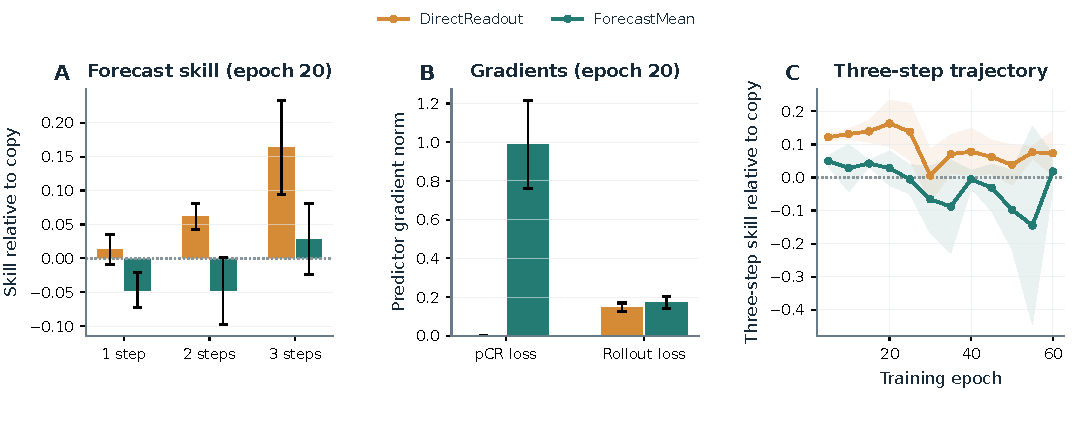
\includegraphics[width=\textwidth]{figures/forecast_mechanism.pdf}
\caption{Archived fixed-training-probe diagnostics across four seeds. (A) Copy-normalized forecast skill at common epoch 20. (B) Predictor gradient norms from pCR and weighted rollout losses. (C) Three-step skill across epochs with complete diagnostic coverage. Statistics are calculated within each snapshot's EMA coordinates, averaged across folds within seed, and summarized across seeds. Error bars in A and B and shading in C show the descriptive sample SD of the four seed-specific fold means. These are training diagnostics, distinct from pCR probability ensembling; real continuous visit chains are required, and three-step eligibility is only 5--9 patients per probe.}
\label{fig:mechanism}
\end{figure*}

\section{Discussion}
\label{sec:discussion}
\subsection{Separating auxiliary supervision from forecast readout}
Across the four selected seeds, auxiliary future-state supervision increased the direct-readout mean Macro AUROC, AP, and F1, and explicit mean forecast readout increased those means further. These averages preserve unfavorable individual results: auxiliary-supervised direct AUROC was below \nojepa{} at seed 2026, and forecast-mean AUROC was below direct readout at seed 42. A favorable metric average does not imply improvement in every training realization or at every operating point.

The full-versus-\nojepa{} Macro AUROC comparison met both the nine-test principal-family criterion (0.00450) and the all-78 sensitivity criterion (0.03850). Its AP and F1 differences did not meet the principal-family criterion, and no full-versus-direct Macro comparison did so. In the uniform 99,999-resample table, T1 and T2 AUROC comparisons against \nojepa{} also passed secondary-family and all-78 adjustment. However, an independent 999,999-resample check changed the T2 all-78 value from 0.04408 to 0.054872 when the other 77 values were held fixed. The T2 global decision is therefore sensitive to Monte Carlo precision; the check did not repeat the Macro or T1 simulations. These findings support conditional AUROC differences among the selected fitted predictors; they do not independently confirm a general architectural benefit or remove retrospective model and seed selection bias.

The \direct{}--\nojepa{} contrast most closely isolates future-state supervision. The full-versus-direct contrast jointly changes access to predicted state and change features and classifier input width. Classifier-width-matched direct readout, stopped-gradient forecast features, copy-state readout, and independent holdout forecast evaluation would help distinguish these contributions. The main model uses equal spatial weights in its forecast readout while retaining self-attention in the shared Transformers. It predicts embeddings rather than generating MRI for classification. The internal name \nojepa{} denotes removal of future-state supervision while retaining the shared fusion network and transition queries.

\subsection{What additional visits change}
Forecast mean's mean AUROC and F1 peaked at T1, whereas mean AP increased across T0--T2. Its paired T2--T0 intervals included zero for all three metrics. Changes in true- and false-positive predictions explain why more observations, ranking, and a fixed-threshold decision rule need not improve together. Outcome-conditioned histograms summarize probability changes within each seed-specific ensemble; they do not demonstrate that every patient's prediction improves or that score changes are treatment effects.

T0 imaging preceded randomization, while the model is conditioned on the eventual assigned arm. This remains a retrospective conditional scenario. The arm encoding does not capture delivered dose, cycle timing, dose reductions, adherence, or treatment changes. Altering the arm token cannot identify an individual treatment effect without suitable causal assumptions and exposure data. Complete T0--T2 holdout eligibility also restricts the population to which the longitudinal comparison applies.

\subsection{Classification, probability quality, and hypothetical utility}
The additional metrics expose trade-offs behind the ranking means. Compared with auxiliary-supervised direct readout, forecast mean had higher sensitivity, NPV, balanced accuracy, and MCC but lower specificity and slightly lower PPV and accuracy. Neither the sensitivity nor specificity contrast passed secondary-family adjustment. Their point estimates and unadjusted intervals remain relevant descriptions of the selected operating point, rather than multiplicity-adjusted evidence for a clinical benefit or harm. Both direct and forecast-mean accuracy were only marginally above the all-negative reference.

Forecast mean had worse NLL, Brier score, and ECE point estimates than both direct-readout controls. Its higher ranking means therefore did not imply better predicted probabilities. The OOF Youden analysis slightly increased F1 for \nojepa{} but decreased it for the other models. Development OOF scores originate from one held-out fold model per patient, whereas test scores average five models within a seed. Transferring thresholds between these score distributions is a sensitivity analysis rather than independent ensemble calibration.

At the illustrative thresholds 0.30, 0.50, and 0.70, direct readout had higher mean net benefit than forecast mean despite lower AUROC. These are comparisons under a generic positive-action utility, not evaluations of a defined care pathway. A clinically motivated threshold requires consequences for false-positive and false-negative actions to be specified and calibration to be fitted without holdout leakage.

\subsection{Seed variation, subgroups, and forecasting diagnostics}
The mean and sample standard deviation across four seeds describe four training realizations using identical development folds and holdout patients. They do not turn seeds into independent clinical replications. Patient-bootstrap intervals and tests answer a different question: how the mean metric of these fixed predictors varies under patient resampling. Because seeds are not resampled and models are not refitted, those intervals do not estimate uncertainty over the training algorithm or future seed choices.

Subgroup summaries are exploratory, use small denominators, and do not test subtype interactions. The HR-positive/HER2-negative and HR-negative/HER2-negative full-versus-control Macro AUROC intervals excluded zero without multiplicity correction, whereas the other two HR/HER2 intervals included zero. These findings do not establish a corrected subtype-specific benefit. Low sensitivity at 0.5 in the HR-positive/HER2-negative group also persists. Source namespaces share one clinical release and do not provide external validation. The crop subgroup with 11 patients and only one positive outcome cannot support reliable discrimination assessment under the minimum-outcome rule.

Archived fixed-training-probe diagnostics are separate from the pCR holdout analysis. Their copy-normalized skills and gradient norms are calculated in each snapshot's own EMA representation, averaged over folds within seed, and then summarized across seeds. They do not ensemble latent states or establish anatomical forecast fidelity. At epoch 20, auxiliary-supervised direct models had higher mean copy-normalized skill than forecast mean at all three horizons, despite the latter's higher mean pCR AUROC. This weakens an explanation based solely on more accurate forecasts. Gradient routing supports an implementation-level mechanism, but gradient magnitude is not a biological effect size. Independent forecast evaluation at the selected pCR checkpoints remains necessary.

\subsection{Limitations and a confirmatory study}
\label{sec:limitations}
The choice of forecast mean as the overall model and the seed set 42, 44, 71, and 2026 were made after earlier holdout results had been available. This model and reporting-policy change, probability ensembling, and the statistical procedures are retrospective. Patient-bootstrap inference conditions on the fitted ensembles and fixed OOF thresholds. It excludes retraining, overall-model and seed selection, aggregation choice, checkpoint selection, and threshold-selection uncertainty. Four selected seeds do not establish broad training stability, and their sample standard deviations have limited precision. The reported mean describes four five-model predictors; it is not the performance of one twenty-model ensemble or a model trained on the full development cohort.

The 95\% patient intervals are unadjusted. Holm corrections for nine principal and 69 secondary tests, together with the all-78 sensitivity analysis, do not undo retrospective choices. Null-centered bootstrap tests are approximate, with finite-sample limitations particularly for non-smooth statistics such as AP, F1, and binned ECE. The conditional AUROC finding and the absence of adjusted AP/F1 or operating-point differences should remain visible together. Nonsignificance does not establish equivalence. A confirmatory study should lock the overall model, seeds, aggregation, checkpoint and threshold selection, and statistical comparisons before evaluating independent patients.

The holdout is an internal downstream split. Twenty-nine patients had belonged to an earlier development split. Current supervised models were retrained using the new patient-disjoint folds and were not warm-started from those earlier pCR models, but codec and localization-model pretraining have not been fully audited for current-holdout overlap. This prevents a claim that every pipeline stage was evaluated on wholly unseen patients.

Fixed baseline localization and cropping may omit multifocal disease or changes outside the field of view. Geometry and array checks do not establish anatomical registration accuracy. Holdout patients have complete T0--T2 imaging, whereas development retains incomplete histories; missingness, acquisition variation, and subtype prevalence may limit transportability. Archived training probes do not replace best-checkpoint holdout forecast evaluation and have small long-horizon denominators.

The study remains an internal architectural comparison. Matched clinical-only, conventional imaging, and independent longitudinal baselines are still needed, along with external validation, anatomical quality review, and independently assessed calibration. Precise pCR pathology criteria, scan intervals, ethics determination, and upstream provenance also require final documentation before submission.

\section{Conclusion}
Using spatial mean forecast readout and training seeds 42, 44, 71, and 2026, \fullmodel{} had the highest mean AUROC, AP, and F1 among the three reported models. Its Macro AUROC difference from \nojepa{} passed principal-family and all-78 Holm adjustment, and T1 AUROC passed all-78 adjustment in the uniform analysis. The T2 all-78 conclusion crossed 0.05 in the larger Monte Carlo sensitivity check and should be considered numerically sensitive. Macro AP/F1 and full-versus-direct differences did not pass principal-family adjustment. Operating-point, probability-quality, and hypothetical-utility analyses exposed trade-offs. These conditional internal results require independent validation, complete upstream provenance, stronger matched baselines, and prospectively fixed model, training, and statistical policies.

\section*{Data and code availability}
Source imaging collections are available through The Cancer Imaging Archive, subject to their applicable access conditions and licenses. The present derived manifests, processing lineage, and evaluation outputs are retained locally. \todo{Specify the public repository, versioned release, permitted derived-data artifacts, and access mechanism before submission; no public code-release claim is made in this draft.}
\section*{Ethics approval and consent}
\todo{Provide the original studies' ethics and consent statements and the local institutional determination for this secondary analysis, including an approval or exemption identifier where applicable. Public availability alone is not an ethics approval.}
\section*{Funding}
\todo{Provide grant numbers and the funders' roles, or confirm that no specific funding was received.}
\section*{Declaration of competing interest}
\todo{Obtain and insert the actual declarations from every author.}
\section*{CRediT authorship contribution statement}
\todo{Provide author names and agreed contributions; no authorship or contributions have been inferred.}
\section*{Declaration of generative AI and AI-assisted technologies in the manuscript preparation process}
During preparation of this initial draft, OpenAI Codex was used to organize source evidence, generate reproducible aggregate tables and figures, and assist with English drafting. \todo{All authors must review and edit the manuscript, verify every statement and reference, and finalize the disclosure under the journal's current policy before submission.}
\clearpage
\appendix
\section{Supplementary metrics and uncertainty}
\label{sec:supplement}
All three principal models use seeds 42, 44, 71, and 2026 and the same five development folds. Metrics are computed from patient-wise five-fold probability means within each seed and averaged across four seeds. The direct-model results in Table~\ref{tab:seedresults} and forecast-mean results in Table~\ref{tab:seedresults_forecast} preserve the individual realizations underlying the reported mean and sample standard deviation.
\begin{table*}[t]
\centering
\small
\caption{Individual-seed results: patient-level fivefold probability ensembles, each evaluated on the same 175 patients (56 positive). Macro is the mean of three landmark metrics. These seed-specific estimates generate the main table mean and sample SD; they are not independent patient cohorts.}
\label{tab:seedresults}
\begin{tabular}{llrrrr}
\toprule
Model & Seed & Landmark & AUROC & AP & F1 \\
\midrule
NoJEPA & 42 & T0 & 0.7216 & 0.5945 & 0.5217 \\
NoJEPA & 42 & T1 & 0.7176 & 0.5966 & 0.5299 \\
NoJEPA & 42 & T2 & 0.7206 & 0.5957 & 0.5378 \\
NoJEPA & 42 & Macro & 0.7199 & 0.5956 & 0.5298 \\
NoJEPA & 44 & T0 & 0.7275 & 0.5954 & 0.5354 \\
NoJEPA & 44 & T1 & 0.7281 & 0.5981 & 0.5426 \\
NoJEPA & 44 & T2 & 0.7281 & 0.5971 & 0.5469 \\
NoJEPA & 44 & Macro & 0.7279 & 0.5968 & 0.5416 \\
NoJEPA & 71 & T0 & 0.7297 & 0.5761 & 0.5217 \\
NoJEPA & 71 & T1 & 0.7299 & 0.5776 & 0.5333 \\
NoJEPA & 71 & T2 & 0.7312 & 0.5804 & 0.5210 \\
NoJEPA & 71 & Macro & 0.7303 & 0.5781 & 0.5254 \\
NoJEPA & 2026 & T0 & 0.7291 & 0.5933 & 0.5538 \\
NoJEPA & 2026 & T1 & 0.7246 & 0.5921 & 0.5538 \\
NoJEPA & 2026 & T2 & 0.7216 & 0.5894 & 0.5606 \\
NoJEPA & 2026 & Macro & 0.7251 & 0.5916 & 0.5561 \\
DirectReadout & 42 & T0 & 0.7435 & 0.5881 & 0.5321 \\
DirectReadout & 42 & T1 & 0.7461 & 0.6119 & 0.5487 \\
DirectReadout & 42 & T2 & 0.7389 & 0.5914 & 0.5600 \\
DirectReadout & 42 & Macro & 0.7428 & 0.5971 & 0.5469 \\
DirectReadout & 44 & T0 & 0.7372 & 0.6025 & 0.5669 \\
DirectReadout & 44 & T1 & 0.7416 & 0.6115 & 0.5692 \\
DirectReadout & 44 & T2 & 0.7410 & 0.6086 & 0.5672 \\
DirectReadout & 44 & Macro & 0.7399 & 0.6075 & 0.5678 \\
DirectReadout & 71 & T0 & 0.7333 & 0.5831 & 0.5333 \\
DirectReadout & 71 & T1 & 0.7381 & 0.5811 & 0.5289 \\
DirectReadout & 71 & T2 & 0.7360 & 0.5832 & 0.5484 \\
DirectReadout & 71 & Macro & 0.7358 & 0.5825 & 0.5369 \\
DirectReadout & 2026 & T0 & 0.7224 & 0.5991 & 0.5246 \\
DirectReadout & 2026 & T1 & 0.7216 & 0.5997 & 0.5085 \\
DirectReadout & 2026 & T2 & 0.7251 & 0.6069 & 0.5469 \\
DirectReadout & 2026 & Macro & 0.7230 & 0.6019 & 0.5266 \\
\bottomrule
\end{tabular}
\end{table*}

\begin{table*}[t]
\centering
\small
\caption{Individual-seed results: patient-level fivefold probability ensembles, each evaluated on the same 175 patients (56 positive). Macro is the mean of three landmark metrics. These seed-specific estimates generate the main table mean and sample SD; they are not independent patient cohorts.}
\label{tab:seedresults_forecast}
\begin{tabular}{llrrrr}
\toprule
Model & Seed & Landmark & AUROC & AP & F1 \\
\midrule
ForecastMean & 42 & T0 & 0.7425 & 0.6188 & 0.5714 \\
ForecastMean & 42 & T1 & 0.7407 & 0.6170 & 0.5891 \\
ForecastMean & 42 & T2 & 0.7389 & 0.6168 & 0.5672 \\
ForecastMean & 42 & Macro & 0.7407 & 0.6175 & 0.5759 \\
ForecastMean & 44 & T0 & 0.7431 & 0.6088 & 0.5625 \\
ForecastMean & 44 & T1 & 0.7494 & 0.6121 & 0.5865 \\
ForecastMean & 44 & T2 & 0.7471 & 0.6209 & 0.5736 \\
ForecastMean & 44 & Macro & 0.7465 & 0.6139 & 0.5742 \\
ForecastMean & 71 & T0 & 0.7553 & 0.6372 & 0.5926 \\
ForecastMean & 71 & T1 & 0.7580 & 0.6409 & 0.5926 \\
ForecastMean & 71 & T2 & 0.7575 & 0.6401 & 0.5755 \\
ForecastMean & 71 & Macro & 0.7569 & 0.6394 & 0.5869 \\
ForecastMean & 2026 & T0 & 0.7497 & 0.6002 & 0.5692 \\
ForecastMean & 2026 & T1 & 0.7495 & 0.6120 & 0.5600 \\
ForecastMean & 2026 & T2 & 0.7477 & 0.6121 & 0.5714 \\
ForecastMean & 2026 & Macro & 0.7490 & 0.6081 & 0.5669 \\
\bottomrule
\end{tabular}
\end{table*}

\begin{table*}[t]
\centering
\footnotesize
\setlength{\tabcolsep}{5pt}
\caption{All 14 macro metrics for the principal variants: point estimate [95\% patient-bootstrap percentile interval]. Within each of seeds 42,44,71,2026, five fold probabilities are averaged per patient, metrics are computed and averaged over T0--T2, then seed metrics are equally averaged. Threshold-dependent metrics use 0.5. Identical patient resamples preserve pairing across models and landmarks. Entries are marginal model intervals; paired differences are reported separately. Intervals condition on the fitted ensembles and exclude retraining and retrospective selection uncertainty. Downward arrows identify metrics for which lower is better.}
\label{tab:extended_macro}
\begin{tabular}{lccc}
\toprule
Metric & NoJEPA & DirectReadout & ForecastMean \\
\midrule
AUROC & 0.7258 [0.6410, 0.8000] & 0.7354 [0.6504, 0.8079] & 0.7483 [0.6675, 0.8194] \\
AP & 0.5905 [0.4683, 0.7057] & 0.5972 [0.4752, 0.7150] & 0.6197 [0.4974, 0.7352] \\
F1 & 0.5382 [0.4297, 0.6323] & 0.5446 [0.4387, 0.6378] & 0.5760 [0.4755, 0.6658] \\
Accuracy & 0.6748 [0.6071, 0.7372] & 0.6814 [0.6138, 0.7434] & 0.6805 [0.6143, 0.7443] \\
Sensitivity & 0.5938 [0.4747, 0.7164] & 0.5967 [0.4784, 0.7155] & 0.6786 [0.5591, 0.7932] \\
Specificity & 0.7129 [0.6362, 0.7873] & 0.7213 [0.6437, 0.7960] & 0.6814 [0.6010, 0.7574] \\
PPV & 0.4941 [0.3800, 0.6059] & 0.5033 [0.3879, 0.6152] & 0.5008 [0.3937, 0.6074] \\
NPV & 0.7891 [0.7097, 0.8643] & 0.7924 [0.7132, 0.8645] & 0.8186 [0.7400, 0.8891] \\
Balanced accuracy & 0.6533 [0.5795, 0.7250] & 0.6590 [0.5870, 0.7299] & 0.6800 [0.6084, 0.7474] \\
MCC & 0.2947 [0.1505, 0.4333] & 0.3066 [0.1634, 0.4435] & 0.3391 [0.2014, 0.4670] \\
Youden index & 0.3066 [0.1589, 0.4500] & 0.3180 [0.1740, 0.4598] & 0.3599 [0.2167, 0.4948] \\
NLL $\downarrow$ & 0.5812 [0.5274, 0.6405] & 0.5771 [0.5218, 0.6387] & 0.5829 [0.5304, 0.6405] \\
Brier score $\downarrow$ & 0.1996 [0.1754, 0.2257] & 0.1979 [0.1731, 0.2251] & 0.2002 [0.1765, 0.2257] \\
ECE $\downarrow$ & 0.1157 [0.0875, 0.1820] & 0.1207 [0.0953, 0.1841] & 0.1405 [0.1067, 0.2048] \\
\bottomrule
\end{tabular}
\end{table*}

\begin{table*}[t]
\centering
\small
\caption{Threshold sensitivity analysis: four-seed mean Macro metrics. Each seed uses landmark-specific Youden thresholds from its disjoint validation-fold scores. OOF single-model scores differ from test fivefold ensemble scores; this is sensitivity analysis, not independent ensemble calibration. No test labels choose thresholds.}
\label{tab:extended_threshold}
\begin{tabular}{llrrrr}
\toprule
Model & Policy & F1 & Sens. & Spec. & MCC \\
\midrule
NoJEPA & 0.5 & 0.538 & 0.594 & 0.713 & 0.295 \\
NoJEPA & OOF validation Youden & 0.542 & 0.615 & 0.694 & 0.295 \\
\midrule
DirectReadout & 0.5 & 0.545 & 0.597 & 0.721 & 0.307 \\
DirectReadout & OOF validation Youden & 0.542 & 0.588 & 0.728 & 0.305 \\
\midrule
ForecastMean & 0.5 & 0.576 & 0.679 & 0.681 & 0.339 \\
ForecastMean & OOF validation Youden & 0.574 & 0.652 & 0.710 & 0.344 \\
\bottomrule
\end{tabular}
\end{table*}


\subsection{Paired significance checks}
Table~\ref{tab:bootstrap} reports the nine principal Macro comparisons, with unadjusted 95\% paired patient-bootstrap intervals, raw two-sided approximate bootstrap $p$ values, within-family Holm adjustment, and all-78 Holm adjustment. The secondary family comprises 69 tests in Tables~\ref{tab:significance_landmarks}--\ref{tab:significance_longitudinal}. Every patient draw is shared across all four fixed seeds, models, and landmarks; metrics are computed within seeds before averaging. The independent patient count remains 175. A significance marker refers to the stated Holm-adjusted family; ns denotes $p_{\mathrm{Holm}}\geq0.05$. The existing 2,000-resample percentile intervals are unadjusted and are not exact inversions of the 99,999-resample null-centered tests. All testing and reporting choices remain retrospective and exploratory.

\begin{table*}[t]
\centering
\small
\caption{Exploratory landmark comparisons. All metrics use approximate, null-centered paired patient-bootstrap tests (99,999 shared draws across seeds, models, and landmarks). All $p$ values are two-sided. $p_{\mathrm{Holm}}$ adjusts jointly over the 69 secondary tests in Tables~\ref{tab:significance_landmarks}--\ref{tab:significance_longitudinal}. Direct and Mean abbreviate DirectReadout and ForecastMean. $^{*}p_{\mathrm{Holm}}<0.05$, $^{**}p_{\mathrm{Holm}}<0.01$, $^{***}p_{\mathrm{Holm}}<0.001$; ns, not significant after the stated correction. Intervals are unadjusted 95\% patient-bootstrap intervals (2,000 shared draws) and need not agree with adjusted test decisions. All analyses condition on the fixed, retrospectively selected seed42/44/71/2026 ensembles; seeds are not resampled.}
\label{tab:significance_landmarks}
\begin{tabular}{lllrrrc}
\toprule
Comparison & Landmark & Metric & Difference [95\% CI] & $p$ & $p_{\mathrm{Holm}}$ & Sig. \\
\midrule
Direct -- NoJEPA & T0 & AUROC & +0.0071 [-0.0028, +0.0168] & 0.1427 & 1.0000 & ns \\
Direct -- NoJEPA & T0 & AP & +0.0034 [-0.0105, +0.0177] & 0.6257 & 1.0000 & ns \\
Direct -- NoJEPA & T0 & F1 & +0.0061 [-0.0127, +0.0250] & 0.5055 & 1.0000 & ns \\
Direct -- NoJEPA & T1 & AUROC & +0.0118 [+0.0024, +0.0217] & 0.0170 & 1.0000 & ns \\
Direct -- NoJEPA & T1 & AP & +0.0099 [-0.0038, +0.0240] & 0.1656 & 1.0000 & ns \\
Direct -- NoJEPA & T1 & F1 & -0.0011 [-0.0170, +0.0136] & 0.8851 & 1.0000 & ns \\
Direct -- NoJEPA & T2 & AUROC & +0.0099 [-0.0003, +0.0208] & 0.0648 & 1.0000 & ns \\
Direct -- NoJEPA & T2 & AP & +0.0069 [-0.0077, +0.0229] & 0.3744 & 1.0000 & ns \\
Direct -- NoJEPA & T2 & F1 & +0.0140 [-0.0107, +0.0420] & 0.2770 & 1.0000 & ns \\
Mean -- NoJEPA & T0 & AUROC & +0.0206 [+0.0084, +0.0330] & 0.0019 & 0.1241 & ns \\
Mean -- NoJEPA & T0 & AP & +0.0264 [+0.0070, +0.0459] & 0.0093 & 0.5884 & ns \\
Mean -- NoJEPA & T0 & F1 & +0.0407 [+0.0047, +0.0861] & 0.0459 & 1.0000 & ns \\
Mean -- NoJEPA & T1 & AUROC & +0.0243 [+0.0117, +0.0372] & 0.0004 & 0.0248 & * \\
Mean -- NoJEPA & T1 & AP & +0.0294 [+0.0040, +0.0530] & 0.0217 & 1.0000 & ns \\
Mean -- NoJEPA & T1 & F1 & +0.0421 [+0.0067, +0.0827] & 0.0289 & 1.0000 & ns \\
Mean -- NoJEPA & T2 & AUROC & +0.0224 [+0.0100, +0.0353] & 0.0006 & 0.0394 & * \\
Mean -- NoJEPA & T2 & AP & +0.0318 [+0.0089, +0.0560] & 0.0106 & 0.6460 & ns \\
Mean -- NoJEPA & T2 & F1 & +0.0304 [-0.0049, +0.0702] & 0.1080 & 1.0000 & ns \\
Mean -- Direct & T0 & AUROC & +0.0135 [+0.0014, +0.0255] & 0.0326 & 1.0000 & ns \\
Mean -- Direct & T0 & AP & +0.0231 [+0.0036, +0.0428] & 0.0253 & 1.0000 & ns \\
Mean -- Direct & T0 & F1 & +0.0347 [-0.0054, +0.0836] & 0.1160 & 1.0000 & ns \\
Mean -- Direct & T1 & AUROC & +0.0125 [+0.0023, +0.0233] & 0.0213 & 1.0000 & ns \\
Mean -- Direct & T1 & AP & +0.0195 [+0.0021, +0.0381] & 0.0373 & 1.0000 & ns \\
Mean -- Direct & T1 & F1 & +0.0432 [+0.0051, +0.0892] & 0.0397 & 1.0000 & ns \\
Mean -- Direct & T2 & AUROC & +0.0126 [+0.0017, +0.0230] & 0.0231 & 1.0000 & ns \\
Mean -- Direct & T2 & AP & +0.0249 [+0.0046, +0.0483] & 0.0255 & 1.0000 & ns \\
Mean -- Direct & T2 & F1 & +0.0163 [-0.0097, +0.0429] & 0.2332 & 1.0000 & ns \\
\bottomrule
\end{tabular}
\end{table*}

\begin{table*}[t]
\centering
\small
\caption{Exploratory Macro operating and probability-quality comparisons. Differences are first-named minus second-named model; negative Brier, NLL, or ECE differences favor the first model. All metrics use approximate, null-centered paired patient-bootstrap tests (99,999 shared draws across seeds, models, and landmarks). All $p$ values are two-sided. $p_{\mathrm{Holm}}$ adjusts jointly over the 69 secondary tests in Tables~\ref{tab:significance_landmarks}--\ref{tab:significance_longitudinal}. Direct and Mean abbreviate DirectReadout and ForecastMean. $^{*}p_{\mathrm{Holm}}<0.05$, $^{**}p_{\mathrm{Holm}}<0.01$, $^{***}p_{\mathrm{Holm}}<0.001$; ns, not significant after the stated correction. Intervals are unadjusted 95\% patient-bootstrap intervals (2,000 shared draws) and need not agree with adjusted test decisions. All analyses condition on the fixed, retrospectively selected seed42/44/71/2026 ensembles; seeds are not resampled.}
\label{tab:significance_extended}
\begin{tabular}{llrrrc}
\toprule
Comparison & Metric & Difference [95\% CI] & $p$ & $p_{\mathrm{Holm}}$ & Sig. \\
\midrule
Direct -- NoJEPA & Accuracy & +0.0067 [-0.0057, +0.0195] & 0.3164 & 1.0000 & ns \\
Direct -- NoJEPA & Sensitivity & +0.0030 [-0.0176, +0.0212] & 0.7827 & 1.0000 & ns \\
Direct -- NoJEPA & Specificity & +0.0084 [-0.0070, +0.0254] & 0.3236 & 1.0000 & ns \\
Direct -- NoJEPA & PPV & +0.0092 [-0.0065, +0.0263] & 0.2611 & 1.0000 & ns \\
Direct -- NoJEPA & NPV & +0.0033 [-0.0059, +0.0119] & 0.4468 & 1.0000 & ns \\
Direct -- NoJEPA & Balanced accuracy & +0.0057 [-0.0068, +0.0183] & 0.3669 & 1.0000 & ns \\
Direct -- NoJEPA & MCC & +0.0119 [-0.0126, +0.0368] & 0.3291 & 1.0000 & ns \\
Direct -- NoJEPA & Youden index & +0.0114 [-0.0136, +0.0367] & 0.3669 & 1.0000 & ns \\
Direct -- NoJEPA & Brier & -0.0016 [-0.0047, +0.0014] & 0.2913 & 1.0000 & ns \\
Direct -- NoJEPA & NLL & -0.0041 [-0.0109, +0.0028] & 0.2416 & 1.0000 & ns \\
Direct -- NoJEPA & ECE & +0.0050 [-0.0086, +0.0209] & 0.4434 & 1.0000 & ns \\
Mean -- NoJEPA & Accuracy & +0.0057 [-0.0195, +0.0319] & 0.6755 & 1.0000 & ns \\
Mean -- NoJEPA & Sensitivity & +0.0848 [+0.0396, +0.1398] & 0.0017 & 0.1096 & ns \\
Mean -- NoJEPA & Specificity & -0.0315 [-0.0603, -0.0057] & 0.0258 & 1.0000 & ns \\
Mean -- NoJEPA & PPV & +0.0067 [-0.0260, +0.0401] & 0.6776 & 1.0000 & ns \\
Mean -- NoJEPA & NPV & +0.0295 [+0.0080, +0.0555] & 0.0133 & 0.7968 & ns \\
Mean -- NoJEPA & Balanced accuracy & +0.0267 [+0.0005, +0.0566] & 0.0650 & 1.0000 & ns \\
Mean -- NoJEPA & MCC & +0.0444 [-0.0053, +0.1028] & 0.1036 & 1.0000 & ns \\
Mean -- NoJEPA & Youden index & +0.0533 [+0.0010, +0.1132] & 0.0650 & 1.0000 & ns \\
Mean -- NoJEPA & Brier & +0.0007 [-0.0052, +0.0063] & 0.8226 & 1.0000 & ns \\
Mean -- NoJEPA & NLL & +0.0017 [-0.0108, +0.0142] & 0.7867 & 1.0000 & ns \\
Mean -- NoJEPA & ECE & +0.0249 [+0.0042, +0.0340] & 0.0104 & 0.6460 & ns \\
Mean -- Direct & Accuracy & -0.0010 [-0.0248, +0.0238] & 0.9526 & 1.0000 & ns \\
Mean -- Direct & Sensitivity & +0.0818 [+0.0404, +0.1327] & 0.0013 & 0.0851 & ns \\
Mean -- Direct & Specificity & -0.0399 [-0.0663, -0.0165] & 0.0019 & 0.1241 & ns \\
Mean -- Direct & PPV & -0.0025 [-0.0322, +0.0288] & 0.8708 & 1.0000 & ns \\
Mean -- Direct & NPV & +0.0262 [+0.0066, +0.0503] & 0.0174 & 1.0000 & ns \\
Mean -- Direct & Balanced accuracy & +0.0210 [-0.0041, +0.0486] & 0.1135 & 1.0000 & ns \\
Mean -- Direct & MCC & +0.0325 [-0.0146, +0.0866] & 0.1939 & 1.0000 & ns \\
Mean -- Direct & Youden index & +0.0419 [-0.0082, +0.0973] & 0.1135 & 1.0000 & ns \\
Mean -- Direct & Brier & +0.0023 [-0.0020, +0.0068] & 0.3234 & 1.0000 & ns \\
Mean -- Direct & NLL & +0.0059 [-0.0040, +0.0158] & 0.2551 & 1.0000 & ns \\
Mean -- Direct & ECE & +0.0199 [-0.0039, +0.0282] & 0.0456 & 1.0000 & ns \\
\bottomrule
\end{tabular}
\end{table*}

\begin{table*}[t]
\centering
\small
\caption{Exploratory paired T2 minus T0 comparisons. Shared patient-bootstrap draws retain dependence between seeds and landmarks. All metrics use approximate, null-centered paired patient-bootstrap tests (99,999 shared draws across seeds, models, and landmarks). All $p$ values are two-sided. $p_{\mathrm{Holm}}$ adjusts jointly over the 69 secondary tests in Tables~\ref{tab:significance_landmarks}--\ref{tab:significance_longitudinal}. Direct and Mean abbreviate DirectReadout and ForecastMean. $^{*}p_{\mathrm{Holm}}<0.05$, $^{**}p_{\mathrm{Holm}}<0.01$, $^{***}p_{\mathrm{Holm}}<0.001$; ns, not significant after the stated correction. Intervals are unadjusted 95\% patient-bootstrap intervals (2,000 shared draws) and need not agree with adjusted test decisions. All analyses condition on the fixed, retrospectively selected seed42/44/71/2026 ensembles; seeds are not resampled.}
\label{tab:significance_longitudinal}
\begin{tabular}{llrrrc}
\toprule
Model & Metric & Difference [95\% CI] & $p$ & $p_{\mathrm{Holm}}$ & Sig. \\
\midrule
NoJEPA & AUROC & -0.0016 [-0.0064, +0.0029] & 0.4961 & 1.0000 & ns \\
NoJEPA & AP & +0.0008 [-0.0080, +0.0092] & 0.8367 & 1.0000 & ns \\
NoJEPA & F1 & +0.0084 [-0.0040, +0.0237] & 0.2390 & 1.0000 & ns \\
DirectReadout & AUROC & +0.0011 [-0.0034, +0.0057] & 0.6268 & 1.0000 & ns \\
DirectReadout & AP & +0.0043 [-0.0057, +0.0137] & 0.3729 & 1.0000 & ns \\
DirectReadout & F1 & +0.0164 [-0.0117, +0.0528] & 0.2999 & 1.0000 & ns \\
ForecastMean & AUROC & +0.0002 [-0.0054, +0.0061] & 0.9513 & 1.0000 & ns \\
ForecastMean & AP & +0.0062 [-0.0063, +0.0194] & 0.3221 & 1.0000 & ns \\
ForecastMean & F1 & -0.0020 [-0.0125, +0.0095] & 0.7162 & 1.0000 & ns \\
\bottomrule
\end{tabular}
\end{table*}


\begin{figure*}[t]
\centering
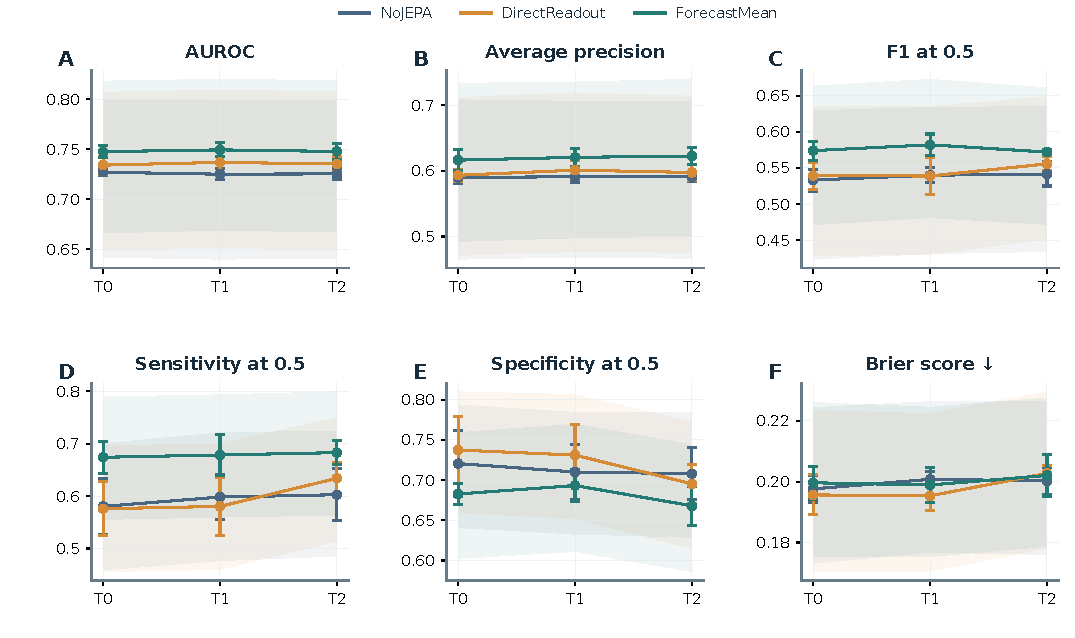
\includegraphics[width=\textwidth]{figures/landmark_performance.pdf}
\caption{Six complementary landmark summaries: AUROC, AP, F1, sensitivity, specificity, and Brier score. Metrics are computed separately from each seed's five-fold ensemble probabilities and then averaged across seeds 42, 44, 71, and 2026. Error bars show descriptive sample seed standard deviations, while shading gives conditional 95\% shared-patient-bootstrap intervals for the seed mean. The same 175 patients appear at every seed and landmark.}
\label{fig:longitudinal}
\end{figure*}

\begin{figure*}[t]
\centering
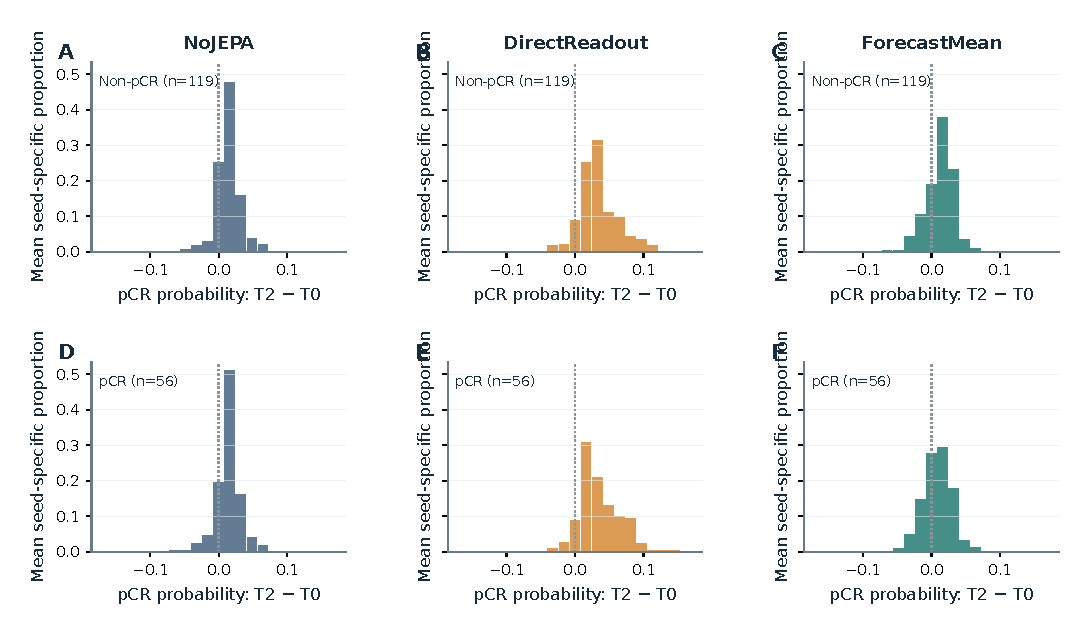
\includegraphics[width=\textwidth]{figures/outcome_score_changes.pdf}
\caption{Outcome-conditioned changes in predicted pCR probability from T0 to T2. For each seed-specific five-fold ensemble, every patient contributes one probability change. Histograms summarize these within-seed changes and are then equally averaged across seeds; probabilities are not averaged across seeds before constructing a change distribution. Panels separate models and outcome classes. Repeated seed predictions are correlated observations of the same 175 patients and do not quadruple the sample size. Score changes do not establish individual treatment effects.}
\label{fig:scorechanges}
\end{figure*}

\section{Supplementary subgroup and training-probe summaries}
\begin{table*}[t]
\centering
\small
\caption{Exploratory subgroup discrimination using seeds 42, 44, 71, and 2026. Within each seed, five fold probabilities are averaged per patient before computing AUROC; Macro averages T0--T2 AUROCs. Model entries are means $\pm$ sample SD across the four seed metrics. Paired patient-bootstrap intervals for the mean ForecastMean minus NoJEPA difference condition on all fitted models and keep the seed set fixed. Age 50 is an exploratory reporting cutpoint. Namespace groups are parts of one clinical release, not external cohorts.}
\label{tab:subgroups}
\begin{tabular}{lrrr}
\toprule
Subgroup ($n$/pCR+) & NoJEPA & Full & $\Delta$ AUROC [95\% interval] \\
\midrule
HR+/HER2- (68/11) & 0.681 $\pm$ 0.016 & 0.720 $\pm$ 0.008 & +0.039 [+0.009, +0.074] \\
HR+/HER2+ (31/12) & 0.637 $\pm$ 0.015 & 0.652 $\pm$ 0.042 & +0.014 [-0.035, +0.063] \\
HR-/HER2+ (14/7) & 0.818 $\pm$ 0.042 & 0.845 $\pm$ 0.022 & +0.027 [-0.027, +0.114] \\
HR-/HER2- (62/26) & 0.634 $\pm$ 0.007 & 0.672 $\pm$ 0.006 & +0.038 [+0.008, +0.070] \\
Age $<$50 (90/29) & 0.670 $\pm$ 0.010 & 0.697 $\pm$ 0.005 & +0.027 [+0.007, +0.047] \\
Age $\geq$50 (85/27) & 0.783 $\pm$ 0.006 & 0.800 $\pm$ 0.009 & +0.016 [+0.000, +0.035] \\
ISPY2 namespace (125/39) & 0.679 $\pm$ 0.002 & 0.705 $\pm$ 0.011 & +0.025 [+0.009, +0.042] \\
ACRIN-6698 namespace (50/17) & 0.847 $\pm$ 0.008 & 0.865 $\pm$ 0.007 & +0.018 [-0.005, +0.042] \\
\bottomrule
\end{tabular}
\end{table*}

\begin{table*}[t]
\centering
\small
\caption{Archived epoch 20 fixed-training-probe diagnostics for seeds 42, 44, 71, and 2026. Each entry is the mean $\pm$ sample SD of four seed-specific five-fold mean skills, distinct from probability ensembling for pCR. Skill is $1-\mathrm{L1}_{forecast}/\mathrm{L1}_{copy}$ within each snapshot\textquotesingle s EMA coordinates; positive is better than holding the landmark state constant. Forecast targets require a continuous actually observed visit chain. These are training-probe summaries, not best-checkpoint holdout forecast evaluations. NoJEPA has no trained-world diagnostic.}
\label{tab:worldprobe}
\begin{tabular}{lrrr}
\toprule
Model & Horizon 1 skill & Horizon 2 skill & Horizon 3 skill \\
\midrule
NoJEPA & -- & -- & -- \\
DirectReadout & +0.013 $\pm$ 0.022 & +0.062 $\pm$ 0.019 & +0.164 $\pm$ 0.070 \\
ForecastMean & -0.047 $\pm$ 0.026 & -0.048 $\pm$ 0.050 & +0.028 $\pm$ 0.052 \\
\bottomrule
\end{tabular}
\end{table*}


\section{Reproducibility and reporting items to complete}
The source package includes aggregate CSV files, source-report hashes, reproducible metric and figure scripts, the shared-patient-bootstrap procedure, and the official article class. The significance CSV includes raw $p$ values, within-family Holm adjustment, and adjustment over all 78 tests as a sensitivity analysis. It contains no patient identifiers, patient-level prediction rows, original MRI volumes, or model checkpoints. The method figure includes only rendered, anonymous development-image slices. Every variant uses training seeds 42, 44, 71, and 2026. Five fold probabilities are averaged per patient within each seed before computing pCR metrics, and seed-specific metric values are then equally averaged. Individual-fold metrics are retained for numerical audit; archived training diagnostics are summarized across folds within seed and then across seeds in their own latent coordinates.

\todo{Before submission, complete author and ethics statements; verify the precise pCR pathology definition; document codec and segmentation patient-level pretraining provenance; add matched external baselines and prospectively locked training and analysis policies; audit external-cohort independence; and confirm the journal's current submission and anonymization requirements.}

\clearpage
\bibliographystyle{elsarticle-harv}
\bibliography{references}
\end{document}
